%%%%%%%%%%%%%%%%%%%%%%%%%%%%%%%%%%%%%%%%%%%%%%%%%%%%%%%%%%%%%%%%%%%%%%%%%%%%%%%%
%% LaTeX Vorlage: ergebnisblatt_vorlage.tex                                   %%
%% Dies ist eine Vorlage fuer die Ergebissblaetter zu den Praktikumsaufagben  %%
%% der Vorlesung 'Einfuehrung in das Wissenschaftliche Rechnen'               %%
%%                                                                            %%
%% Version 2020-04-19, F. Castelli (IANM2, KIT)                               %%
%%%%%%%%%%%%%%%%%%%%%%%%%%%%%%%%%%%%%%%%%%%%%%%%%%%%%%%%%%%%%%%%%%%%%%%%%%%%%%%%
\documentclass[11pt,a4paper]{article}


%% Pakete
\usepackage[ngerman]{babel}
\usepackage[T1]{fontenc}
% \usepackage[utf8]{inputenc}   % Unix
\usepackage[latin1]{inputenc} % Windows
\usepackage[pdftex]{graphicx}
\usepackage{epstopdf}
\usepackage{amsmath,amssymb}


\usepackage{caption}


%% Seitenlayout
\usepackage[DIV=12]{typearea}
\setlength{\parindent}{0em}


%% Font Helvetica
\renewcommand{\rmdefault}{phv}


%% Titelinformationen
\title{Einf\"uhrung in das Wissenschaftliche Rechnen\\
  Praktikumsblatt 4\\
  Aufgabe 7 (Krankheitsausbreitung)}
\author{Lena Hilpp Matr.Nr.: 1941997\\Jan Frithjof Fleischhammer Matr.Nr.: 2115491}
\date{27.05.2020}



%%%%%%%%%%%%%%%%%%%%%%%%%%%%%%%%%%%%%%%%%%%%%%%%%%%%%%%%%%%%%%%%%%%%%%%%%%%%%%%%
\begin{document}
  
  %% Titel
  \maketitle
  
  %%%%%%%%%%%%%%%%%%%%%%%%%%%%%%%%%%%%%%%%%%%%%%%%%%%%%%%%%%%%%%%%%%%%%%%%%%%%%%
  \section*{Problemstellung}
  %%%%%%%%%%%%%%%%%%%%%%%%%%%%%%%%%%%%%%%%%%%%%%%%%%%%%%%%%%%%%%%%%%%%%%%%%%%%%%
  
  In dieser Aufgabe sollte ein SIR-Modell (\textbf{S}usceptible-\textbf{I}nfected-\textbf{R}ecovered) verwendet werden, um die Ausbreitung einer Krankheit zu modellieren.\\
   
  Die Bev\"olkerung wird dabei in Anf\"allige (S), Infizierte (I) und Erholte (R) unterteilt. Dabei gibt es zwei Zustand\"anderungen:
  \begin{itemize}
  \item Infektion: Eine Person geht von S nach I \"uber. Die Infektionsrate wird durch $\beta$ beschrieben.
  \item Heilung / Tod: Eine infizierte Person geht von I nach R. Diese Rate wird durch $\gamma$ beschrieben.
  \end{itemize}
  
  Es wird dabei als Modell-Bev\"olkerung Karlsruhe gew\"ahlt. Die Bev\"olkerung wird in 27 Bezirke unterteilt und eine Matrix $\Phi$ gegeben. $\Phi_{ij}$ gibt dabei den Bev\"olkerungsanteil des Stadtteils $i$ an, der vorrangig in den Stadtteil $j$ pendelt.\\
  
  Wenn durch $N_i$ der Bev\"olkerungszahl von Stadtteil $i$ gegeben ist, beschreibt
  \begin{align*}
  N_i^{tot}=\sum_{m=1}^{27}\Phi_{mi}N_m
  \end{align*}
  die Anzahl der Personen, die im Stadtteil i arbeiten.\\
  Damit erh\"alt man vollendes Differenzialgleichungssystem:
  \begin{align*}
  \begin{split}
  \partial_tS_i(t)&=-\sum_{j=1}^{27}\sum_{k=1}^{27}\beta\Phi_{ij}S_i(t)\frac{\Phi_{kj}I_k(t)}{N_j^{tot}}\\
  \partial_tI_i(t)&=\sum_{j=1}^{27}\sum_{k=1}^{27}\beta\Phi_{ij}S_i(t)\frac{\Phi_{kj}I_k(t)}{N_j^{tot}}-\gamma I_i(t)\\
  \partial_tR_i(t)&=\gamma I_i(t)
  \end{split}
  \end{align*}
  
Dabei beschreibt der Term $\Phi_{ij}S_i(t)$ die Zahl der anf\"alligen Personen aus Stadtteil $i$, die in Stadtteil $j$ arbeiten und der Term $\Phi_{kj}I_k(t)$ die Zahl der infizierten Personen aus Stadtteil $k$, die in Stadtteil $j$ arbeiten.
  
  %%%%%%%%%%%%%%%%%%%%%%%%%%%%%%%%%%%%%%%%%%%%%%%%%%%%%%%%%%%%%%%%%%%%%%%%%%%%%%
  \section*{Ergebnis}
  %%%%%%%%%%%%%%%%%%%%%%%%%%%%%%%%%%%%%%%%%%%%%%%%%%%%%%%%%%%%%%%%%%%%%%%%%%%%%%
  
  Zun\"achst wurde eine Krankheit mit $\beta = 0.5$ und $\gamma = 0.25$ betrachtet.\\
  Zum L\"osen wird das explizite Eulerverfahren mit Schrittweite $1$.\\
  

In Abbildung 1 sieht man den Verlauf der L\"osung, wobei $I=\sum_{i=1}^{27}I_i$, S und R analog.\\

In Abbildung 2 ist der r\"aumliche Verlauf der Krankheit dargestellt.\\

Man sieht, dass die Zahl der Gesamtbev\"olkerung konstant bleibt, was Sinn macht, denn durch Zusammenaddieren des Differentialgleichungssystems erh\"alt man

\begin{align*}
\partial_tN(t)=\partial_tS_i(t)+\partial_tI_i(t)+\partial_tR_i(t)=0
\end{align*}

wobei $N(t)$ die Gesamtbev\"olkerungszahl ist.\\

Nun betrachtet man einen anderen Krankheitserreger mit $\beta = 3.75$ und $\gamma = 0.25$ (etwa Masern ohne Impfungen). Unter Verwendung der gleichen Mathode erh\"alt man Abbildung 3.\\

Die Infiziertenzahl wird schnell stark negativ, was nicht dem Modell entspricht. Dies liegt daran, dass es sich um ein steifes Problem handelt und ein expliziter L\"oser verwendet wurde. Um dieses Problem zu beheben k\"onnte man entweder einen impliziten L\"oser verwenden, oder die Schrittweite verkleinern. Das Ergebnis mit Schrittweite $0.1$ sieht man in Abbildung 4.
  
\begin{figure}
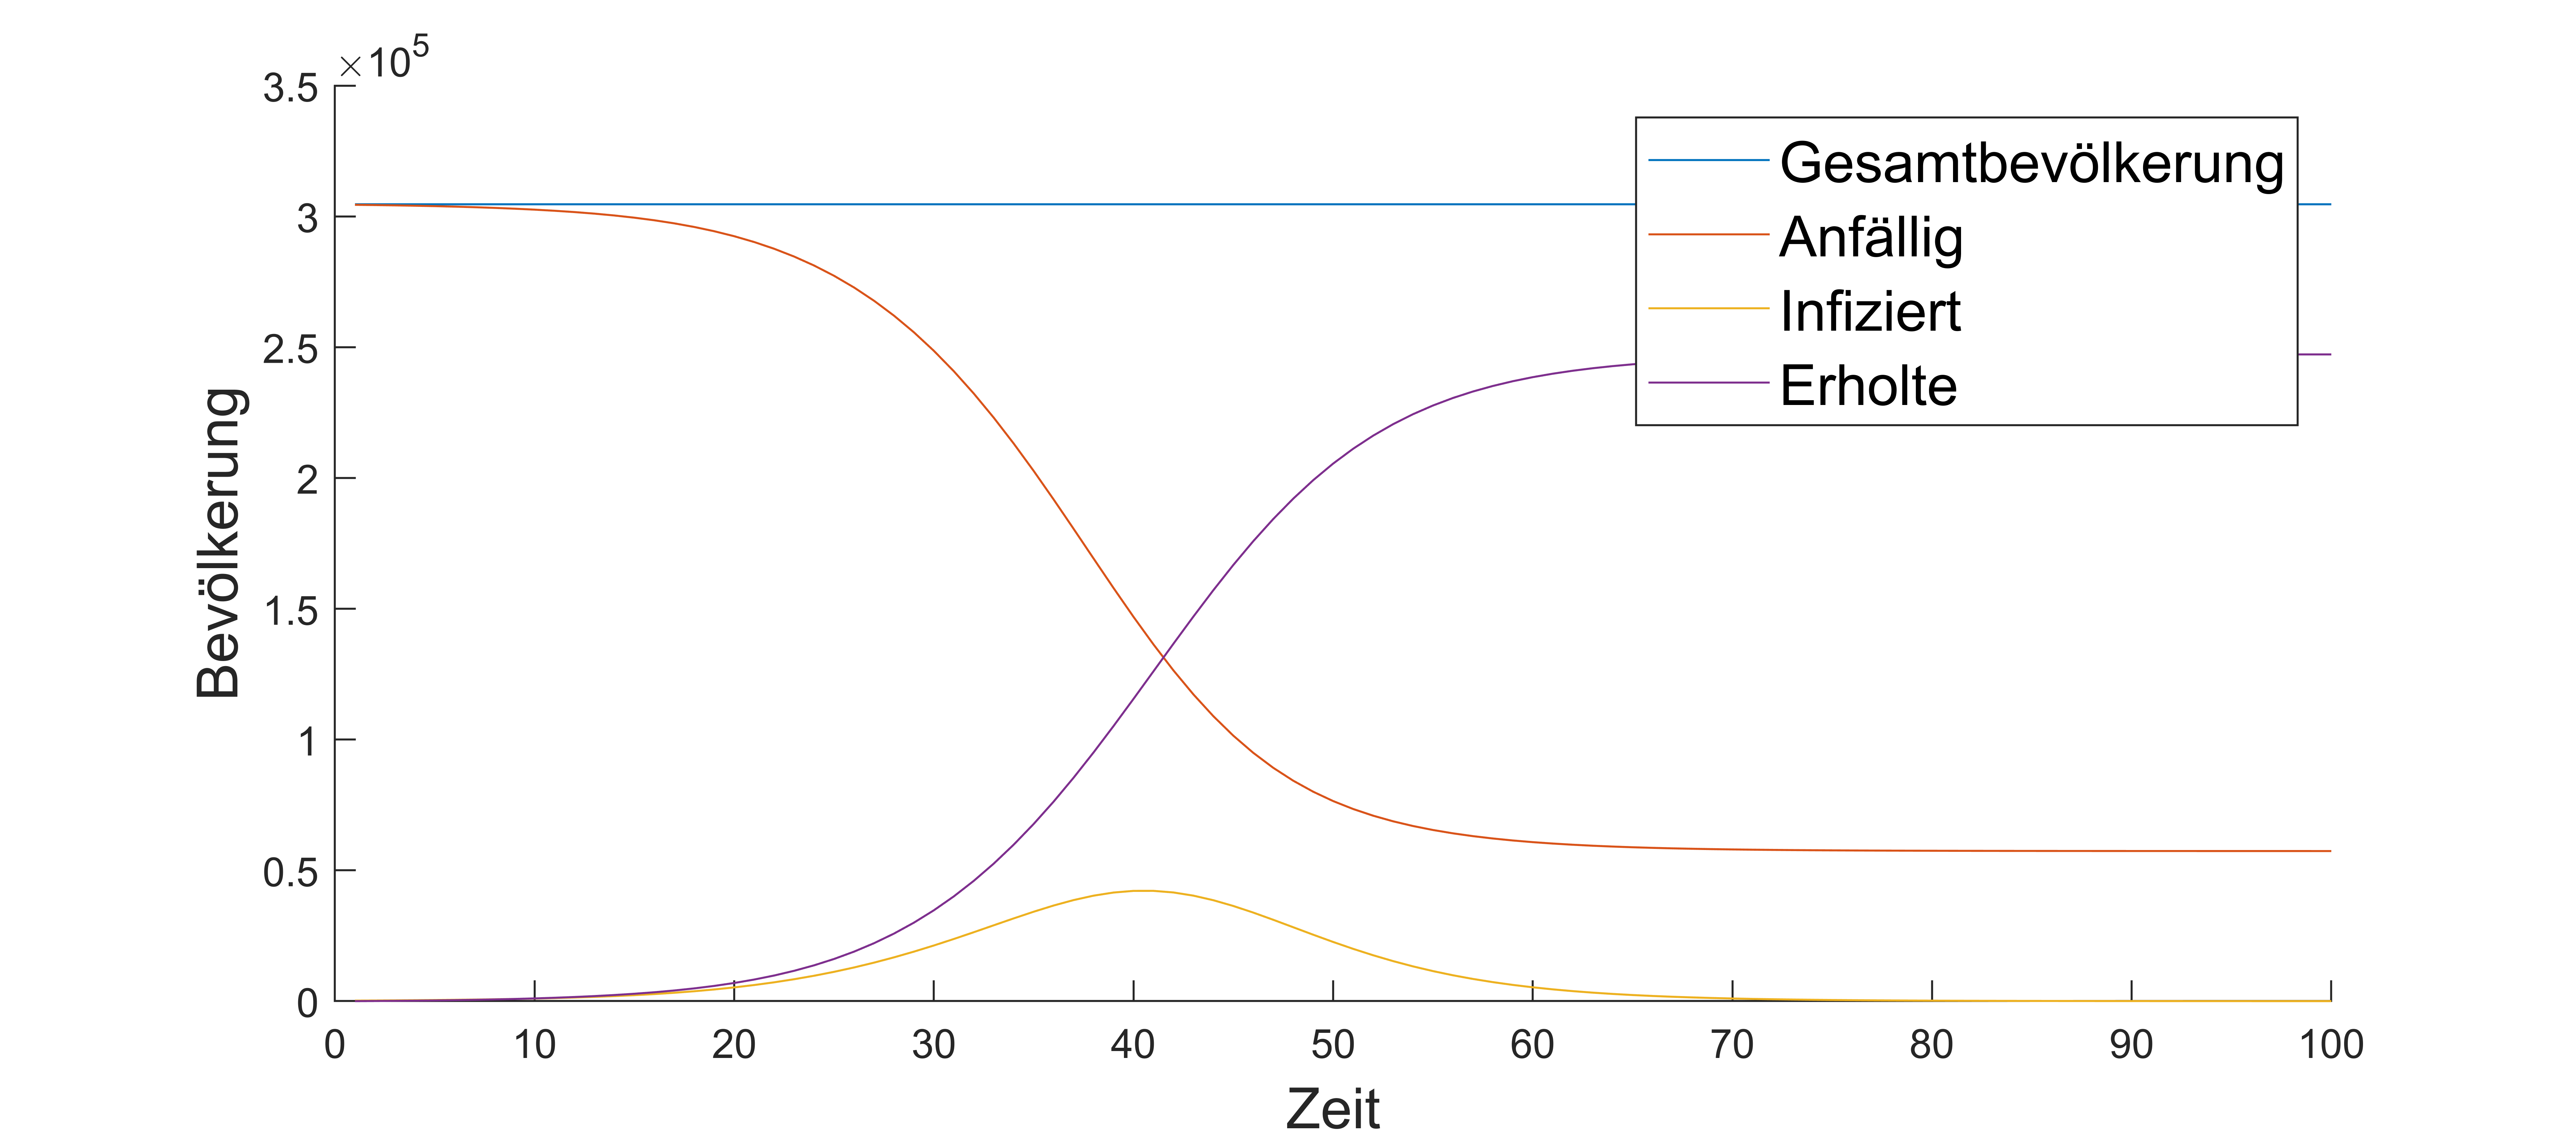
\includegraphics[width=0.8\textwidth]{bild2-1}
\caption{Verlauf der L\"osung}
\end{figure}  

\begin{figure}
\begin{tabular}{ccc}
  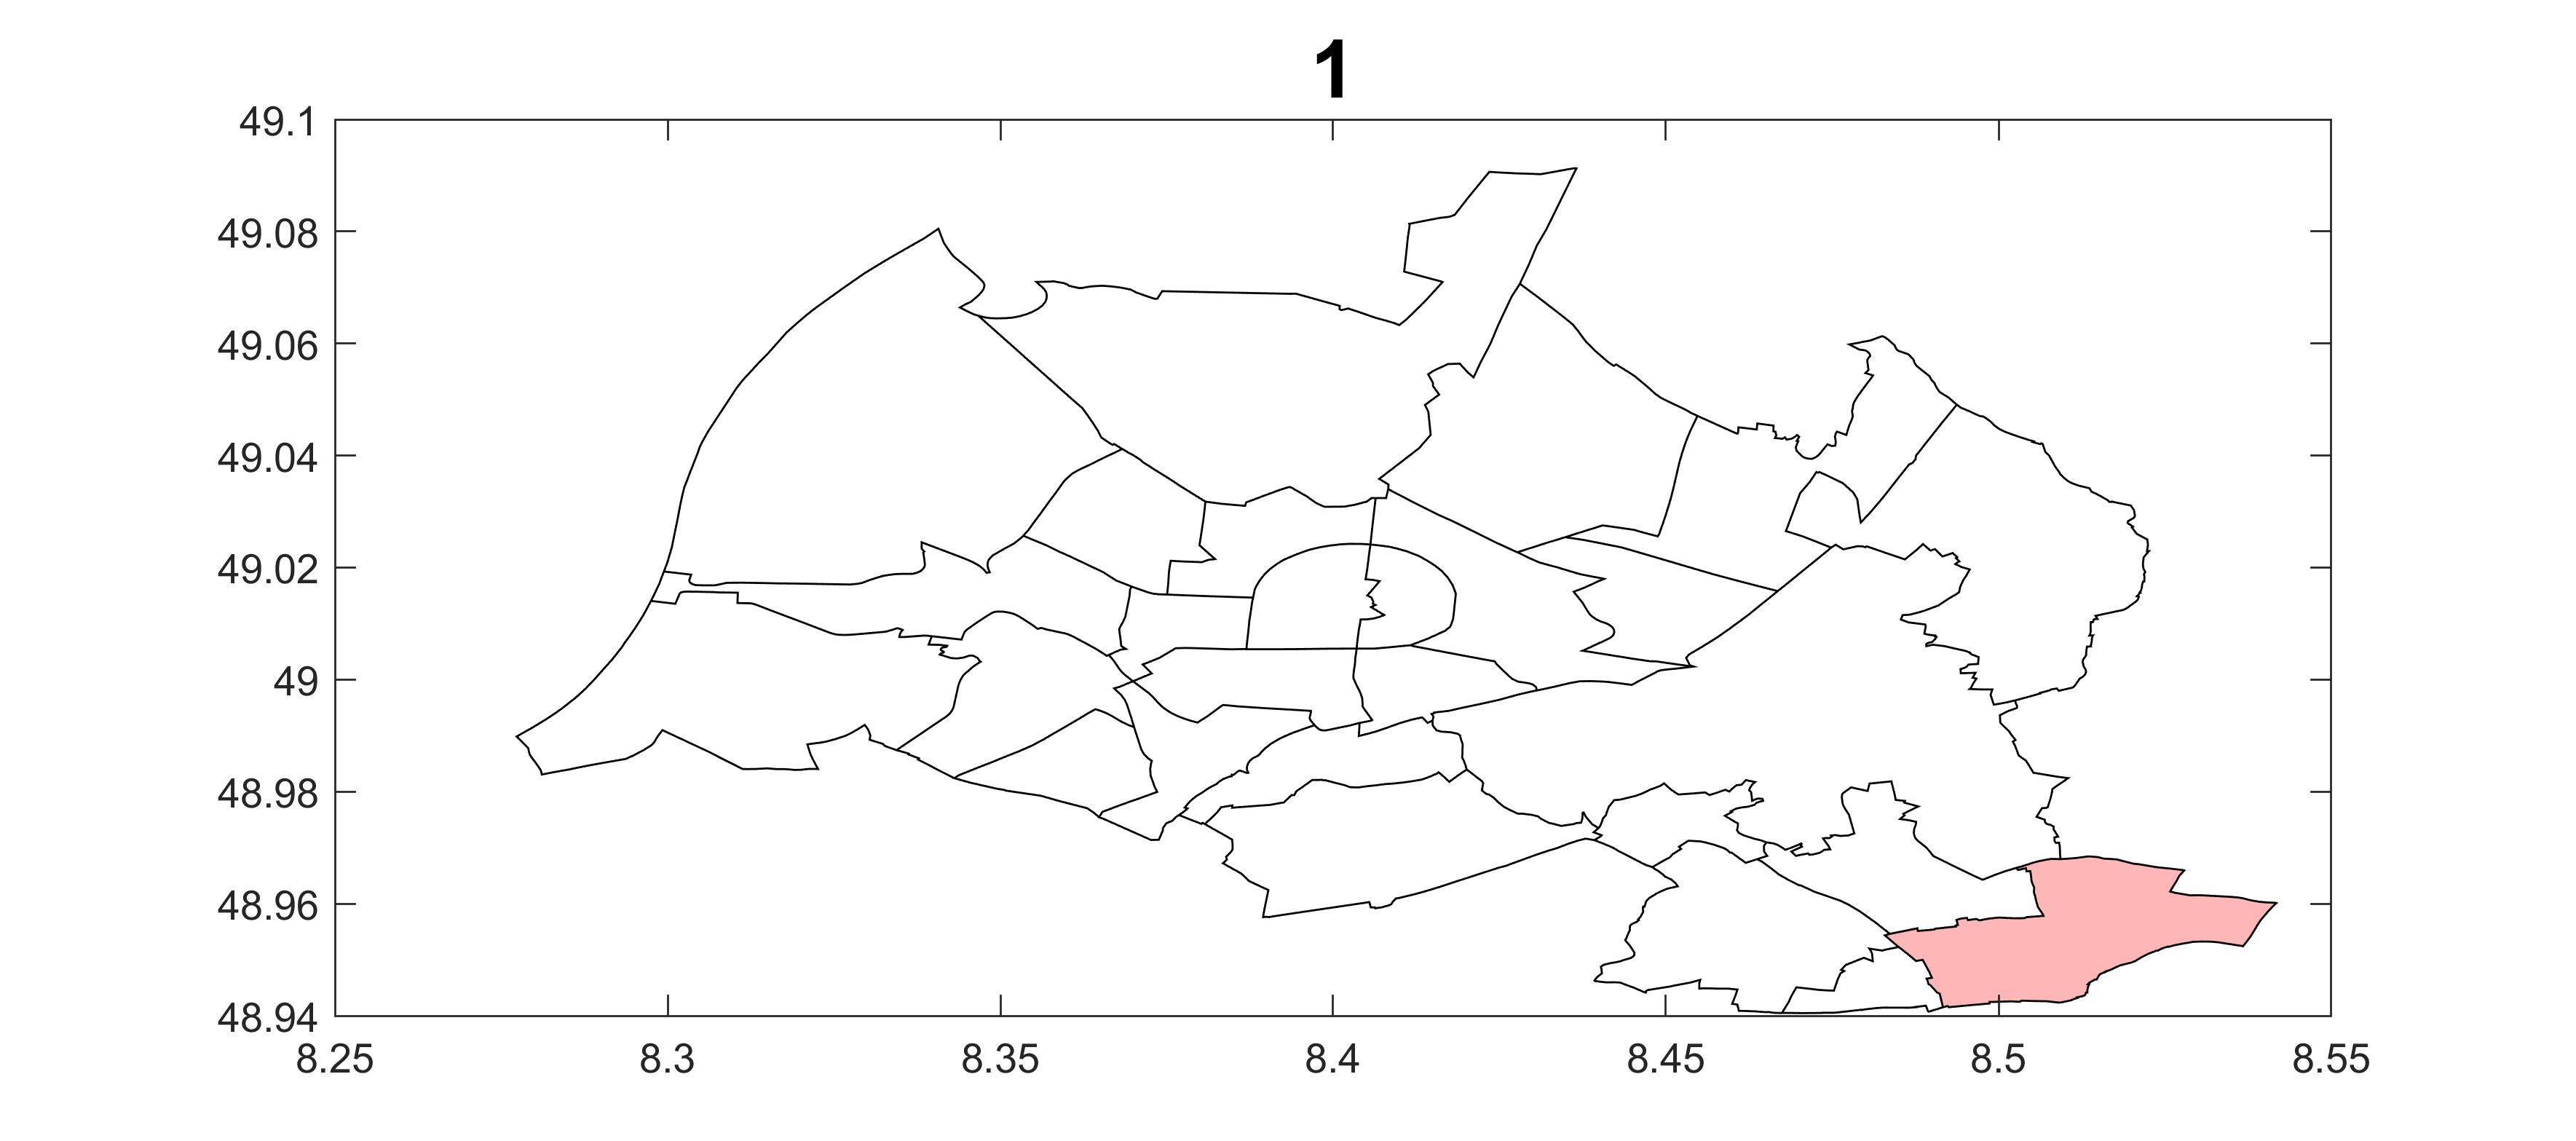
\includegraphics[width=0.3\textwidth]{bild1-1} &
  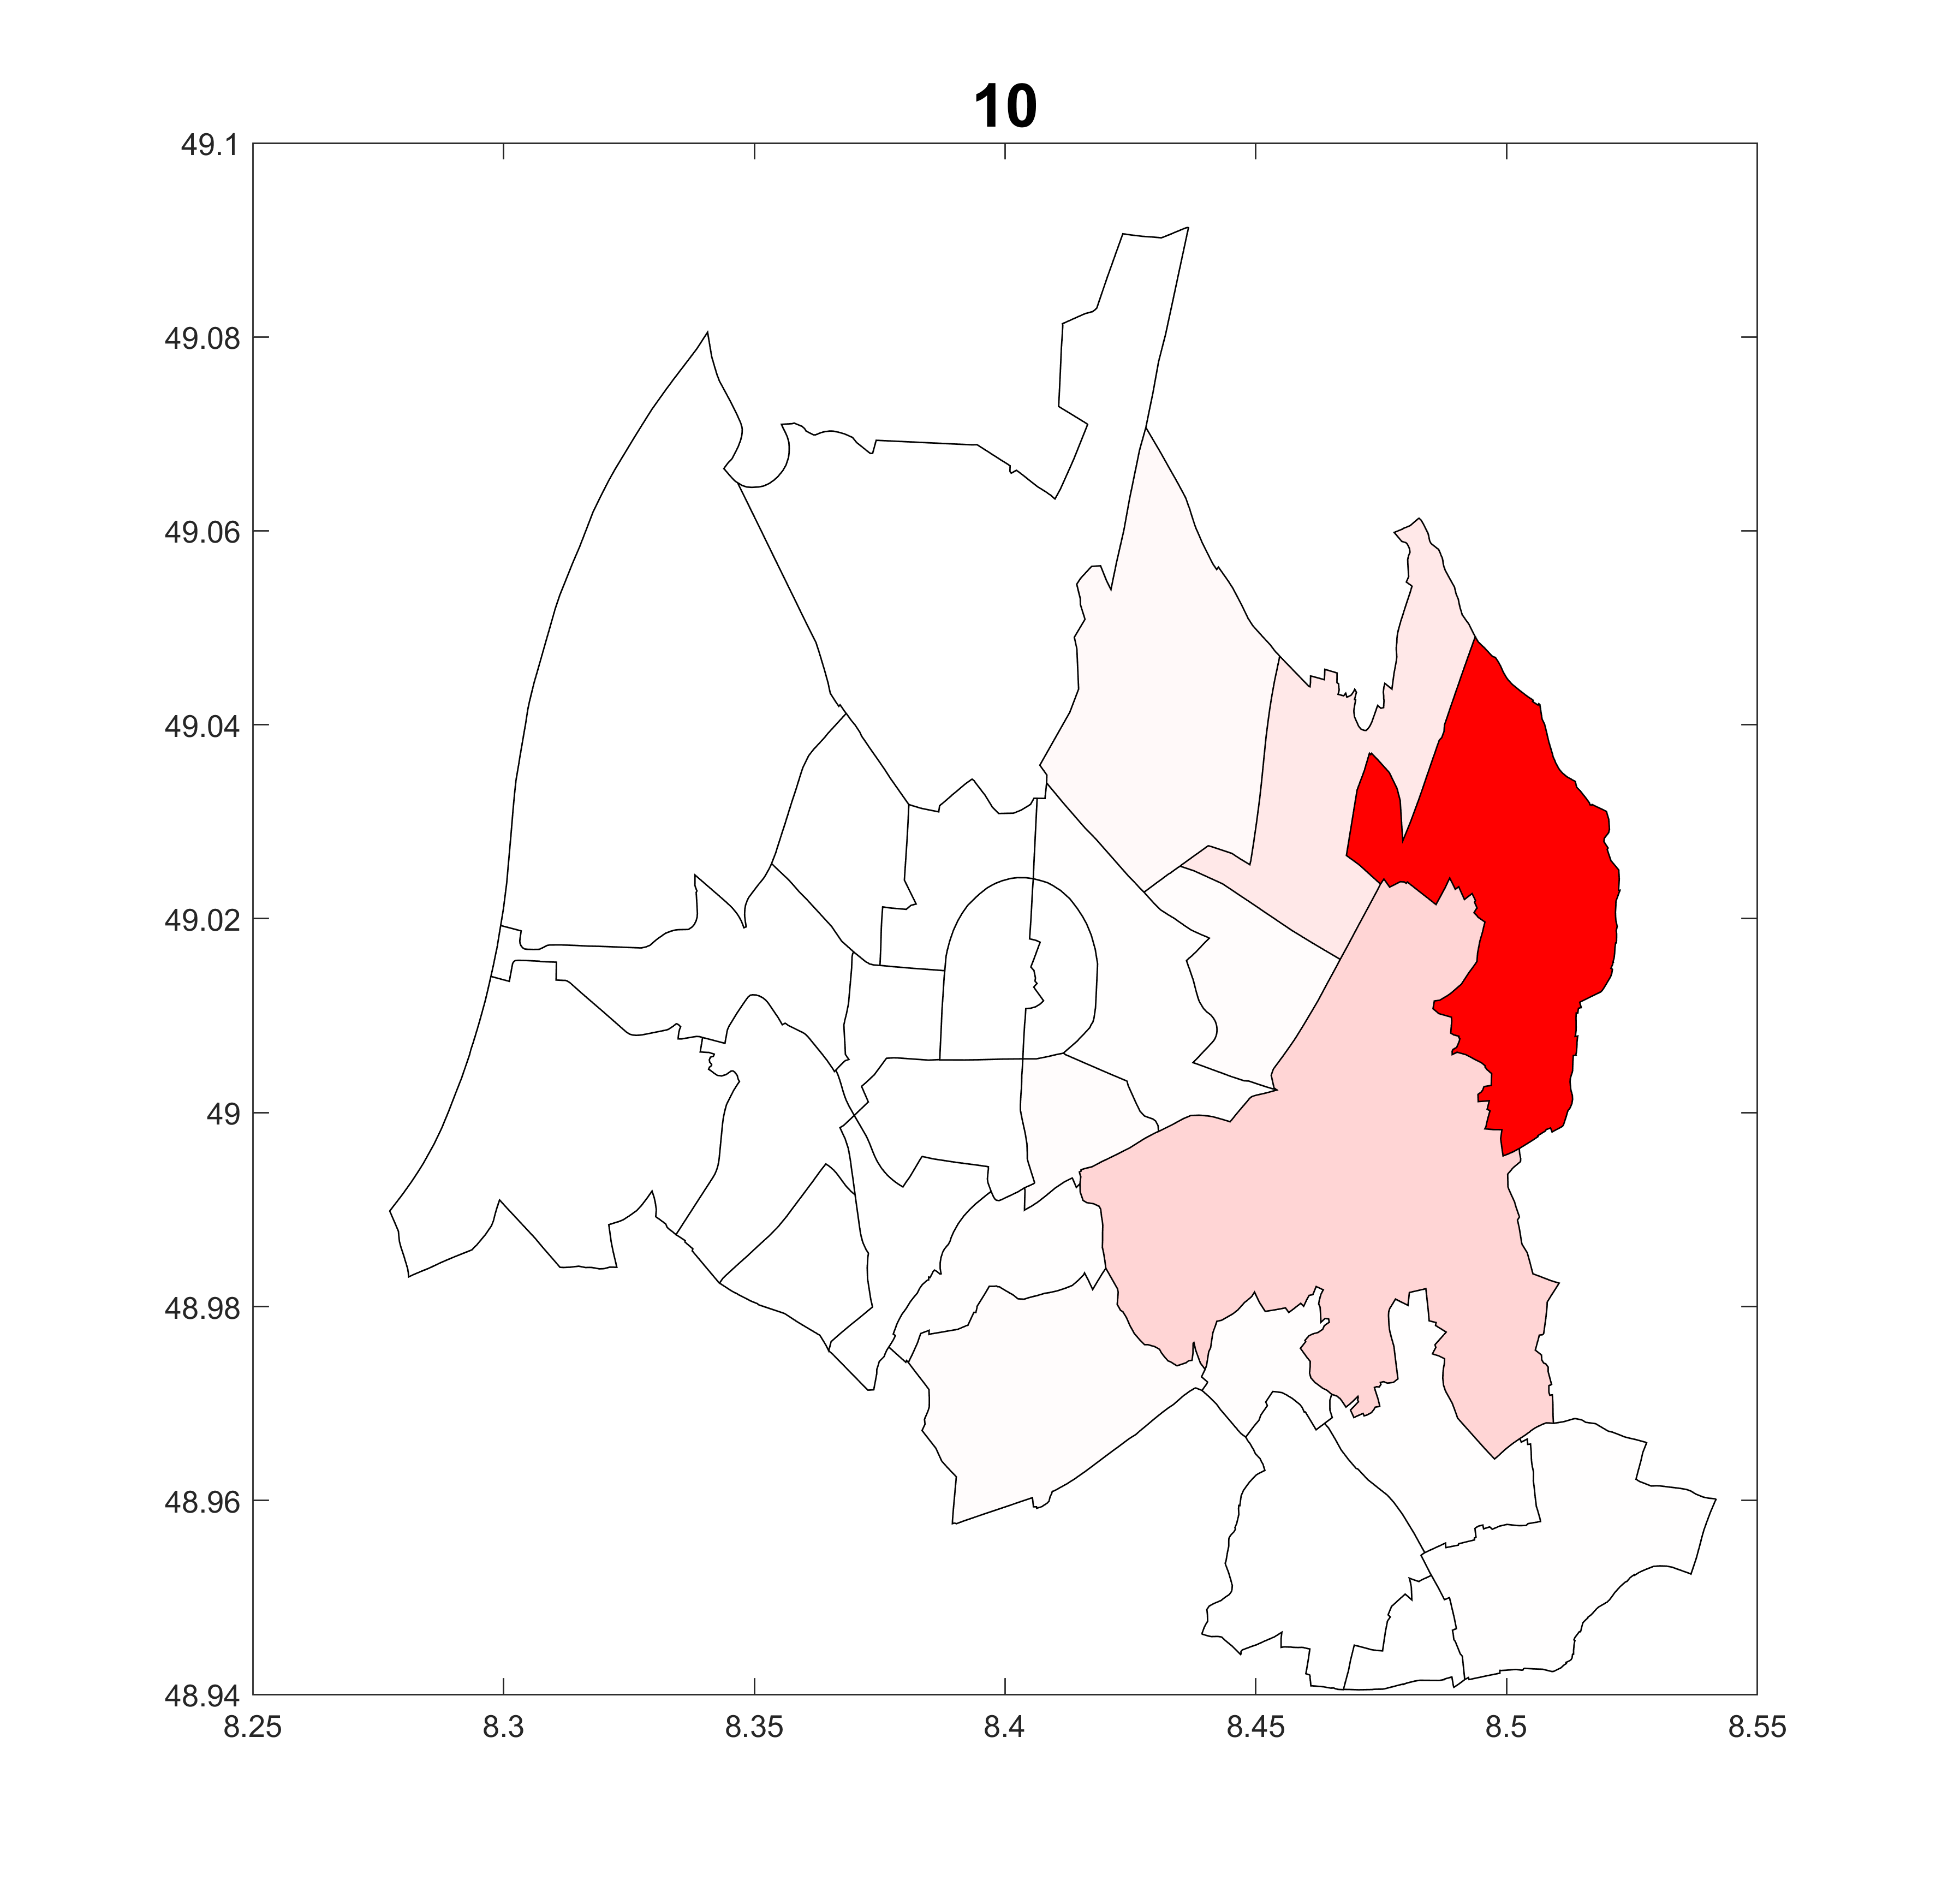
\includegraphics[width=0.3\textwidth]{bild1-10} &
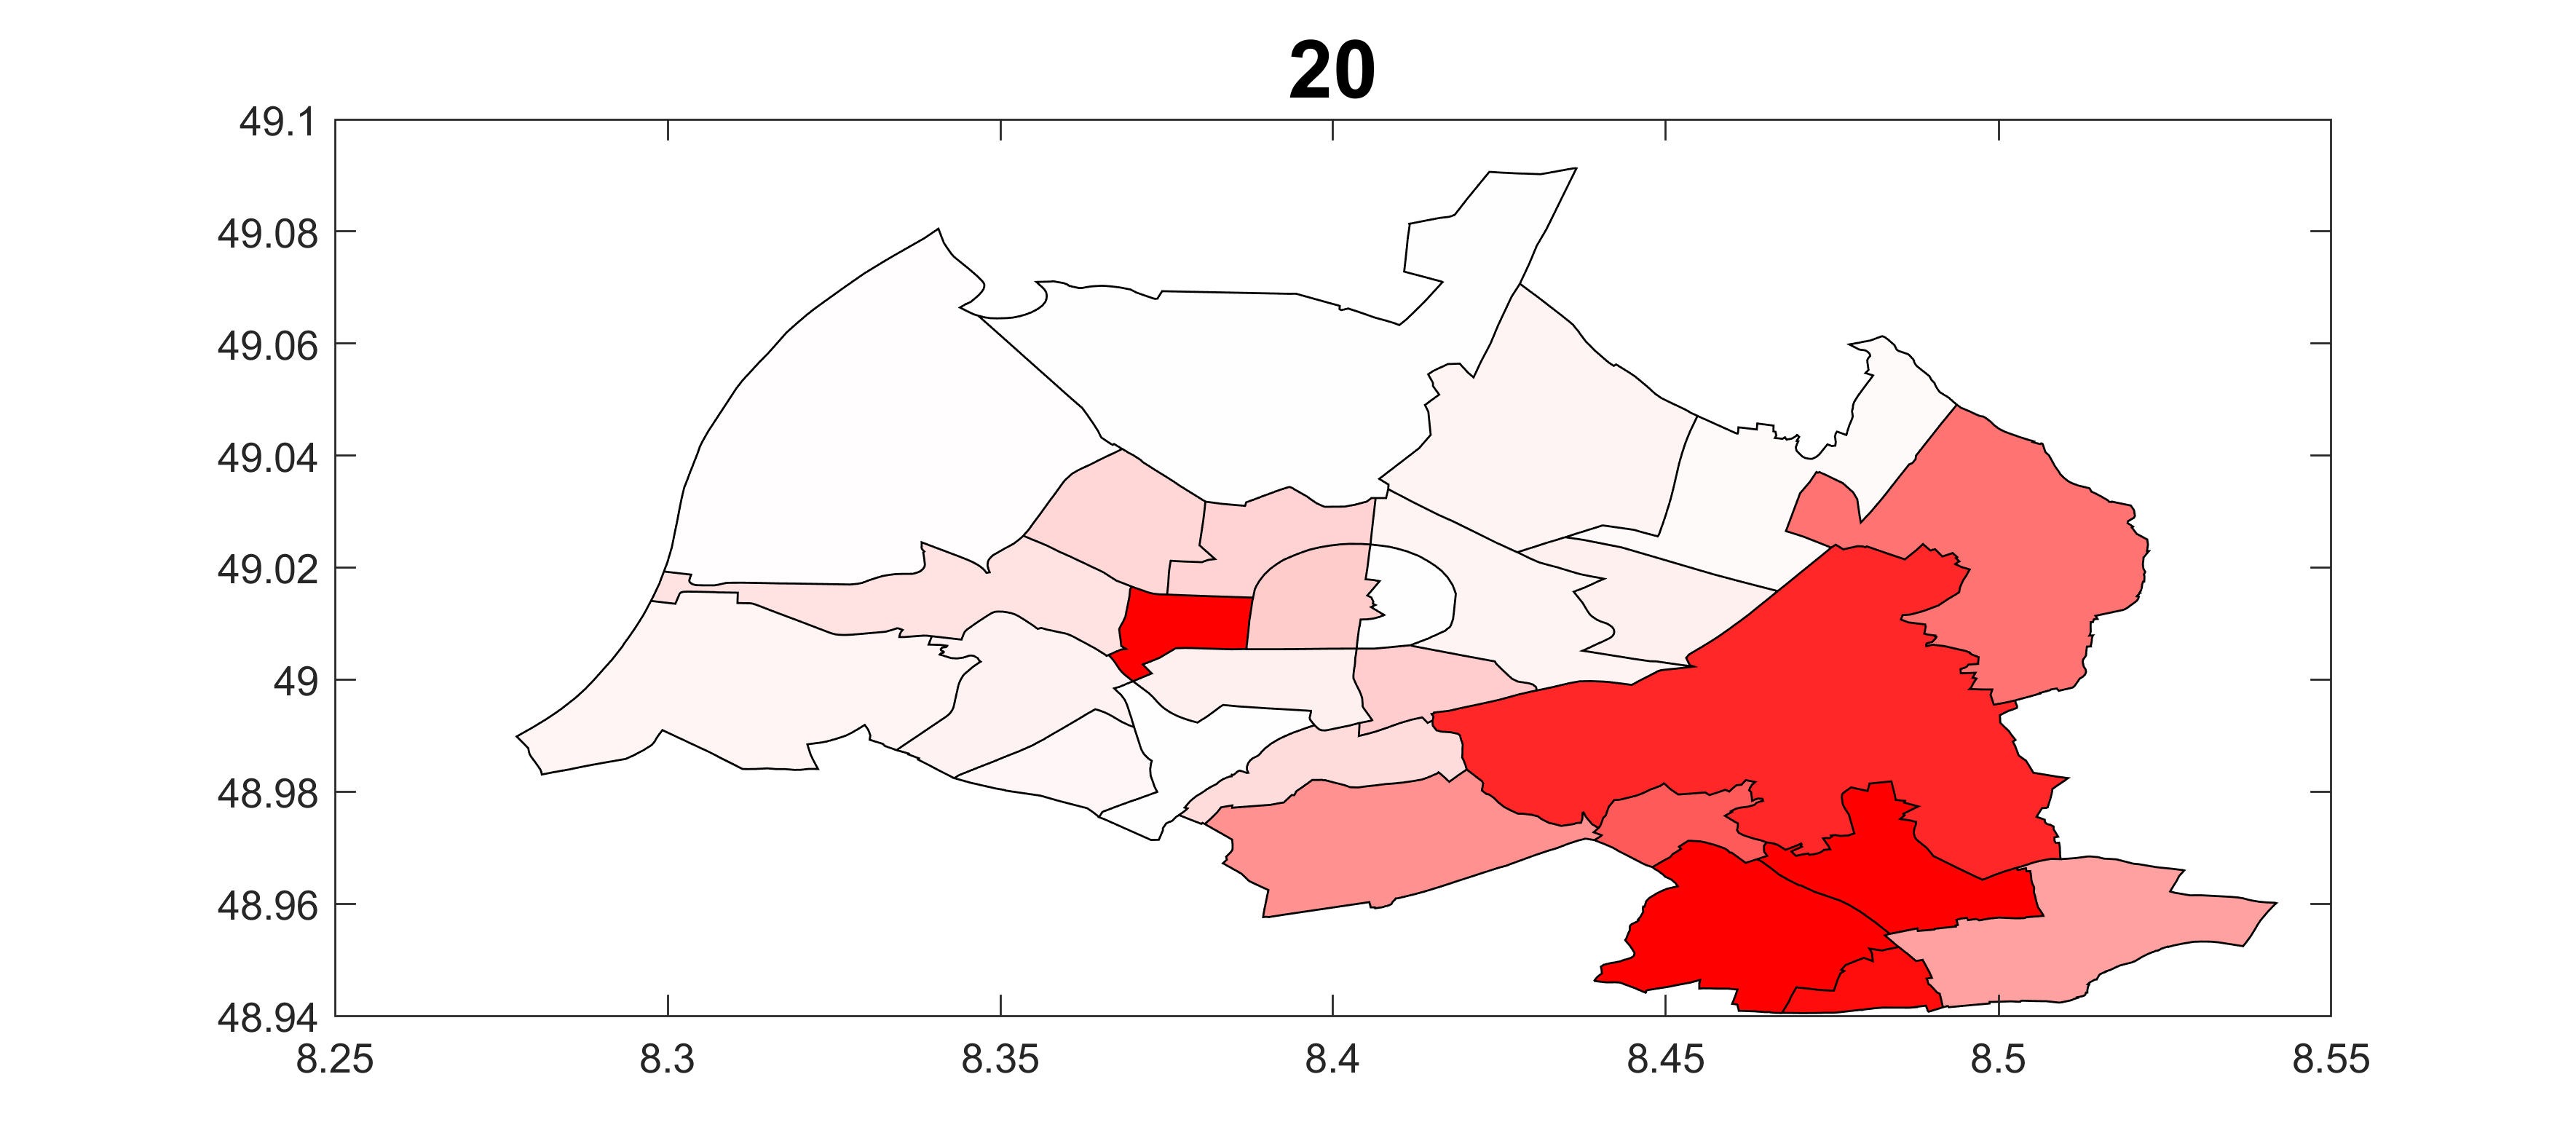
\includegraphics[width=0.3\textwidth]{bild1-20} \\
  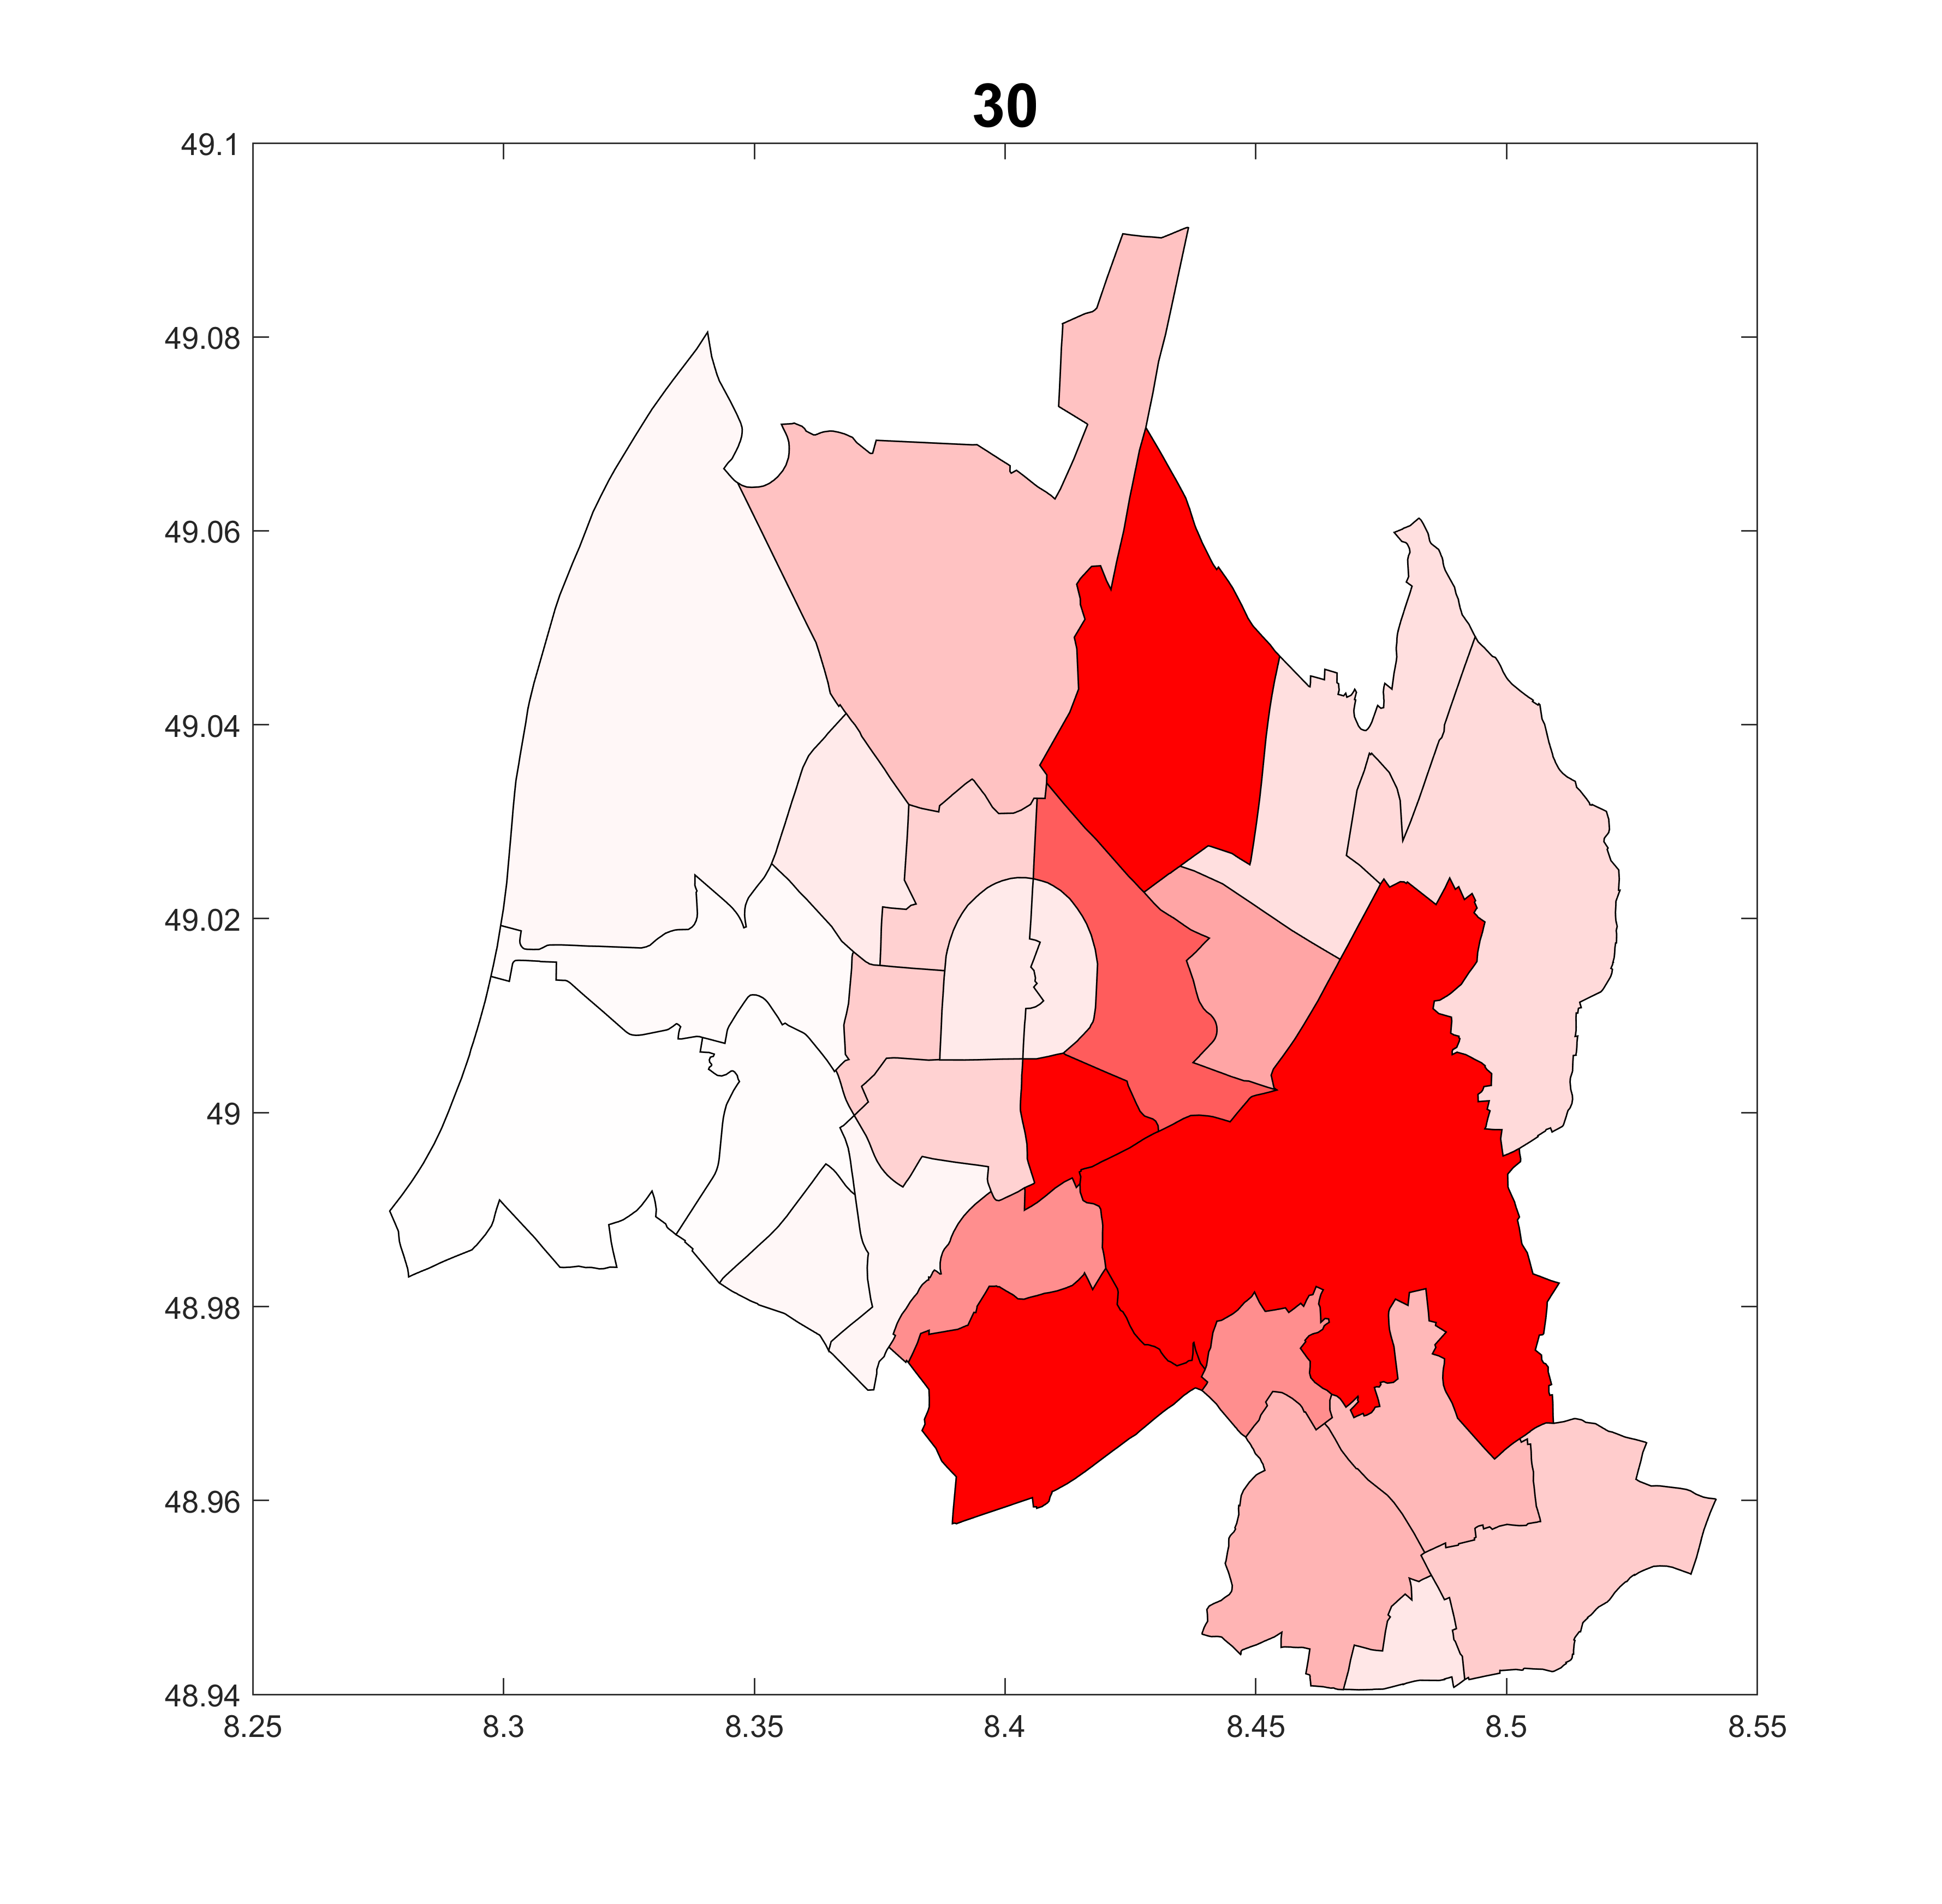
\includegraphics[width=0.3\textwidth]{bild1-30} &
  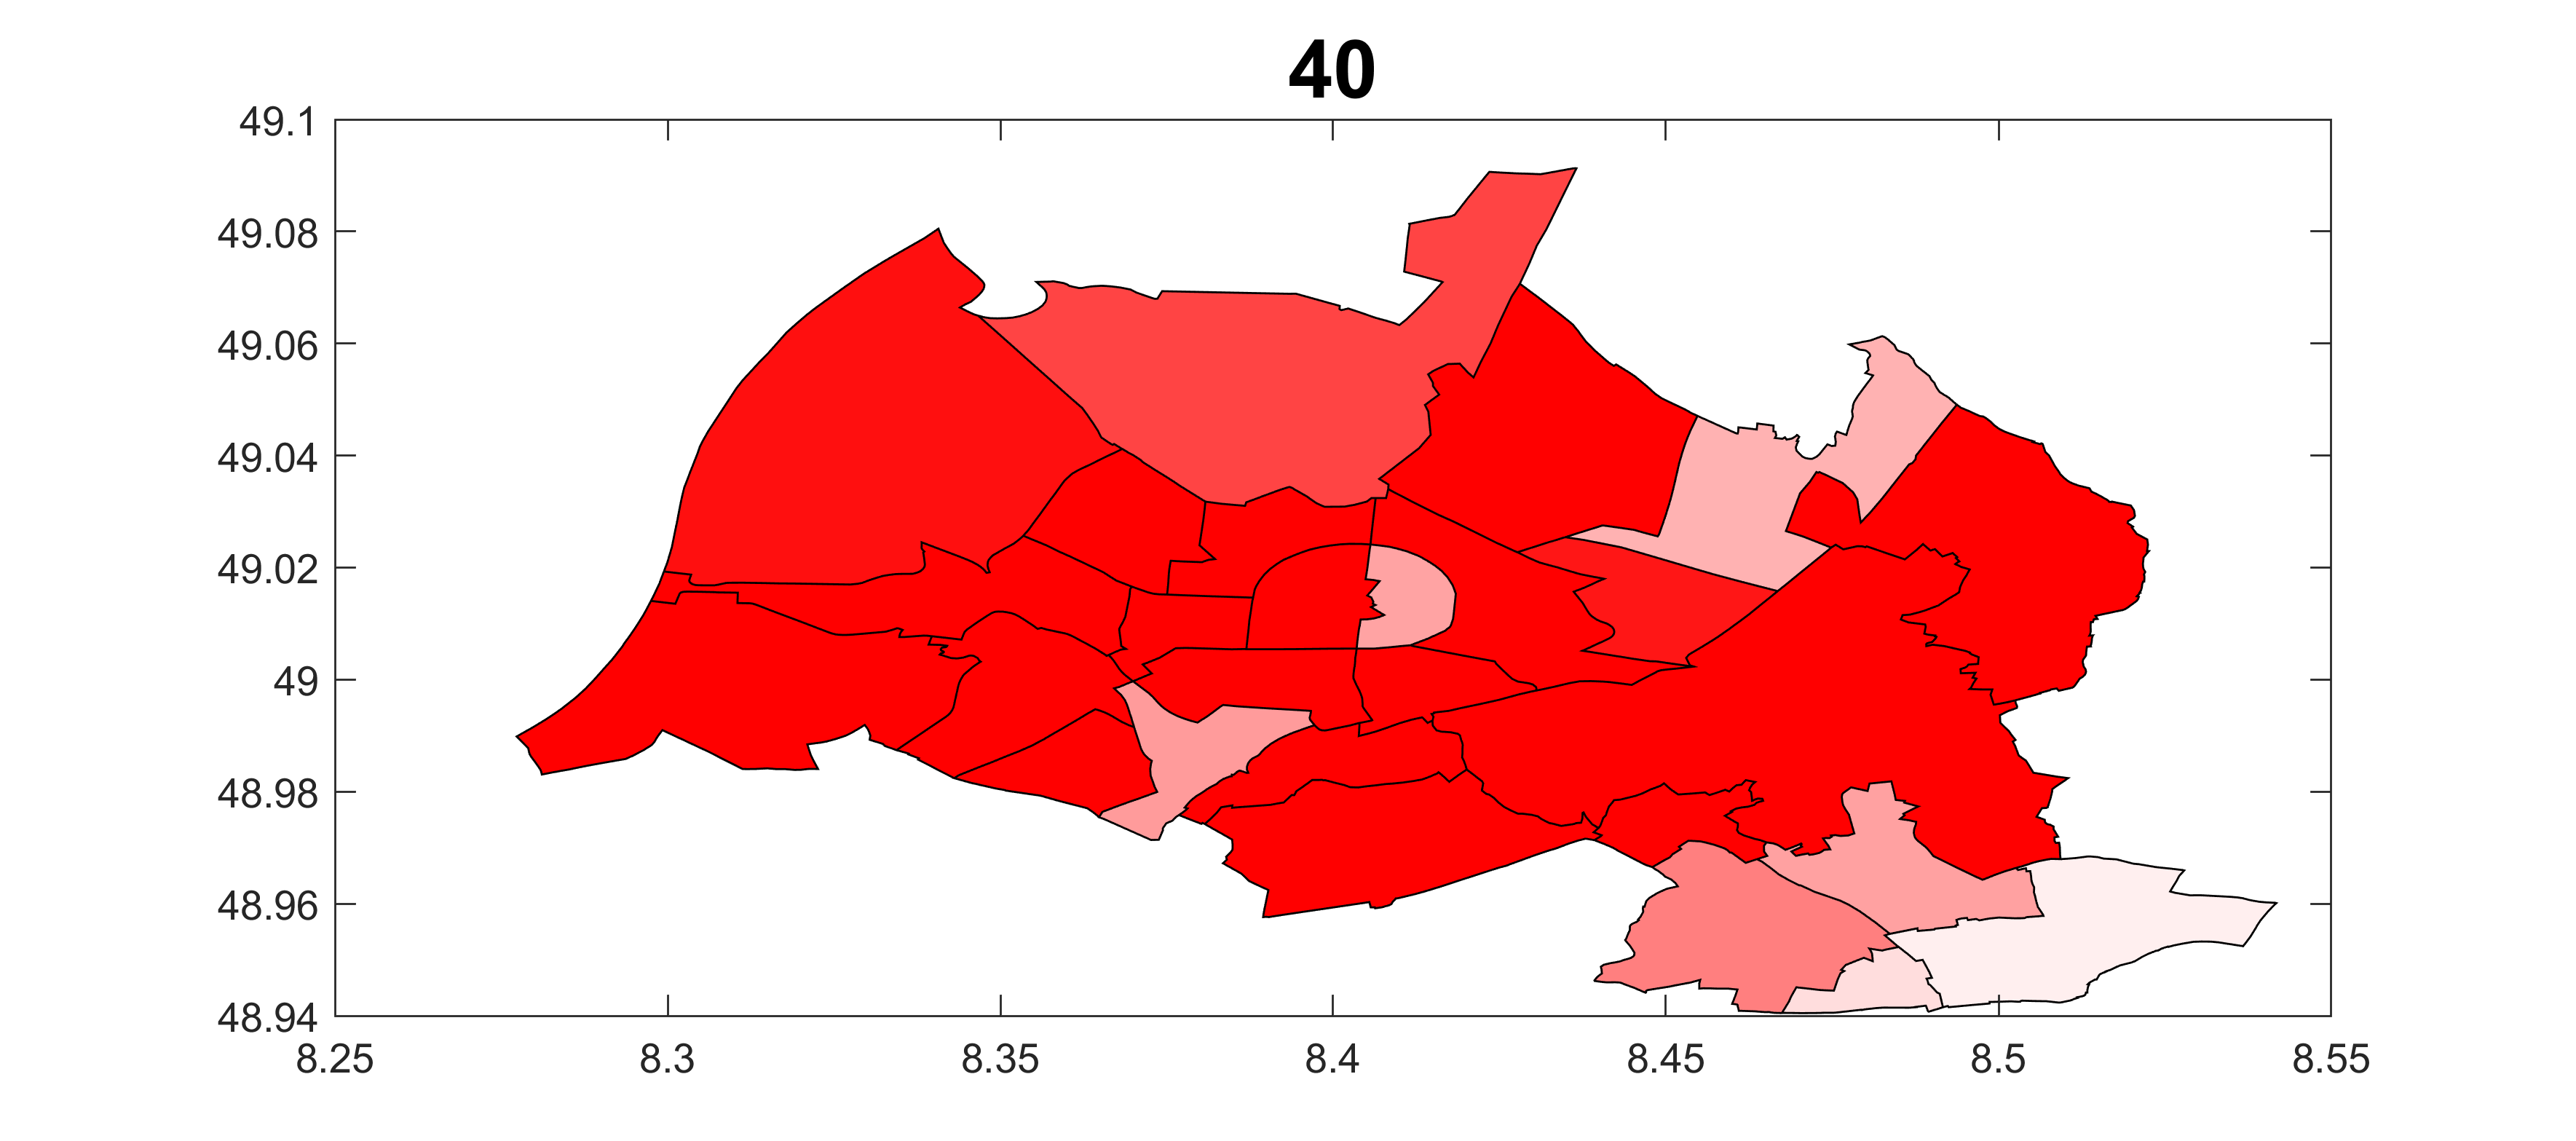
\includegraphics[width=0.3\textwidth]{bild1-40} &
  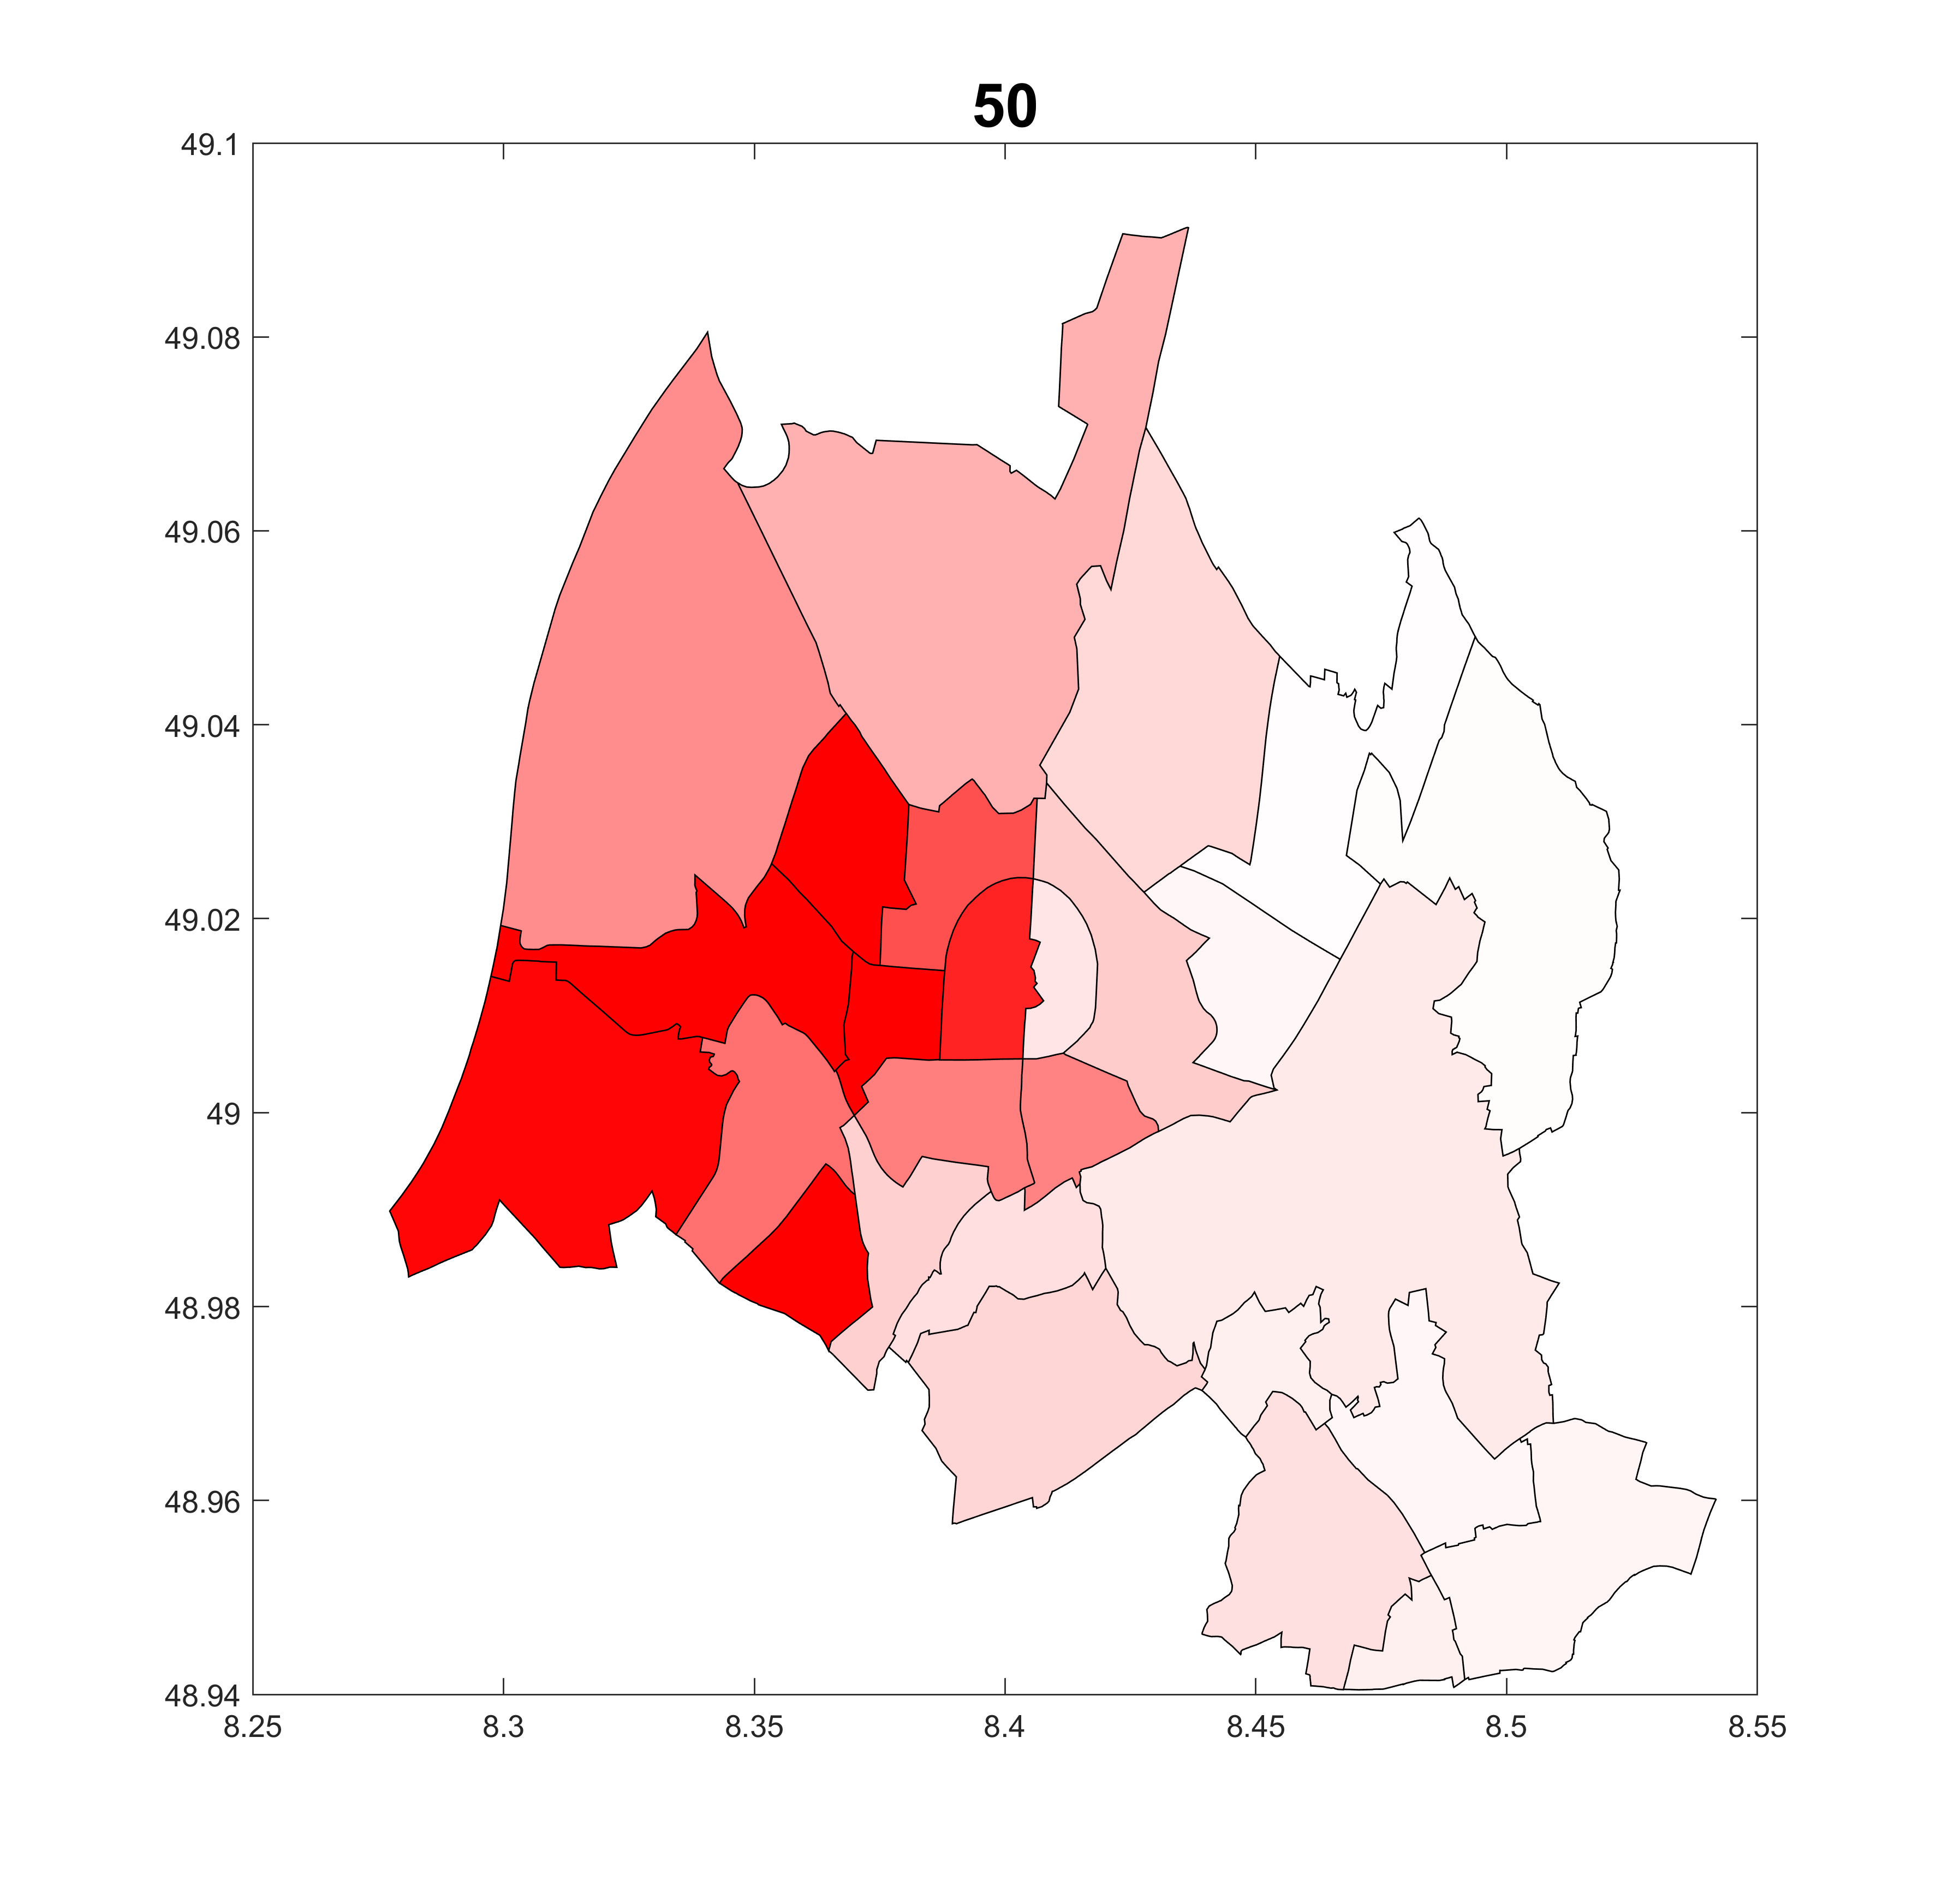
\includegraphics[width=0.3\textwidth]{bild1-50} \\
  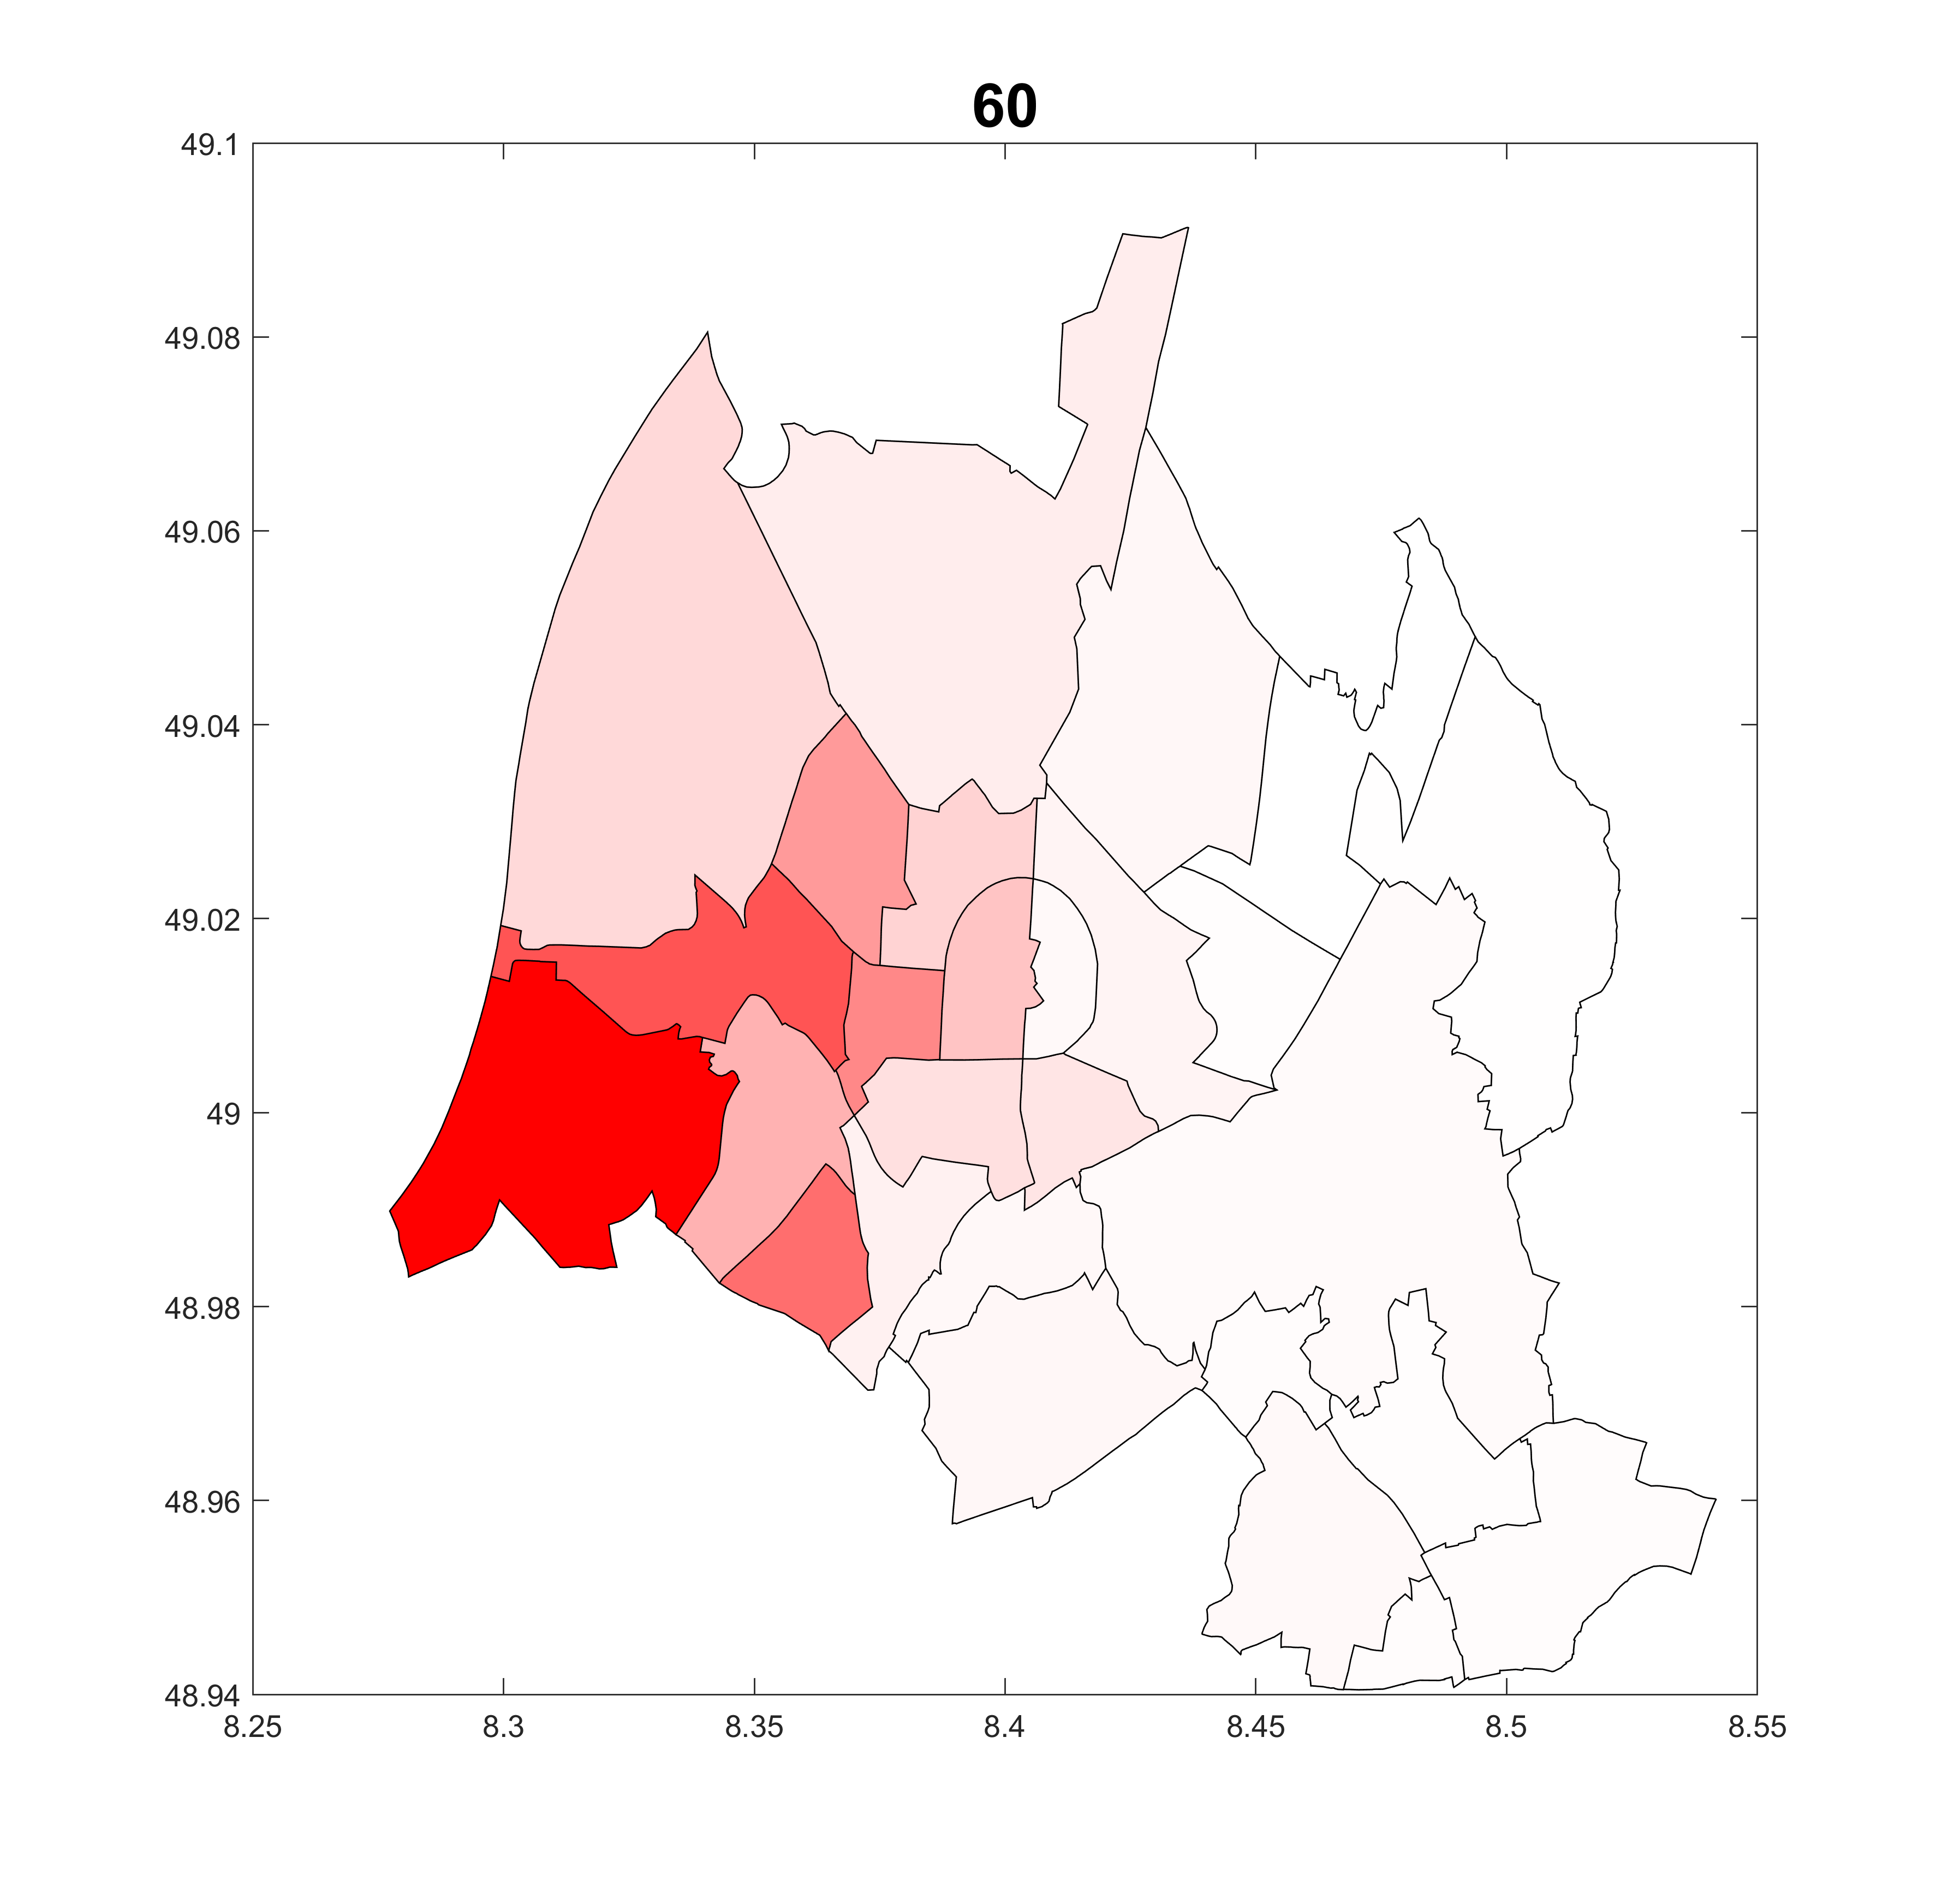
\includegraphics[width=0.3\textwidth]{bild1-60} &  
  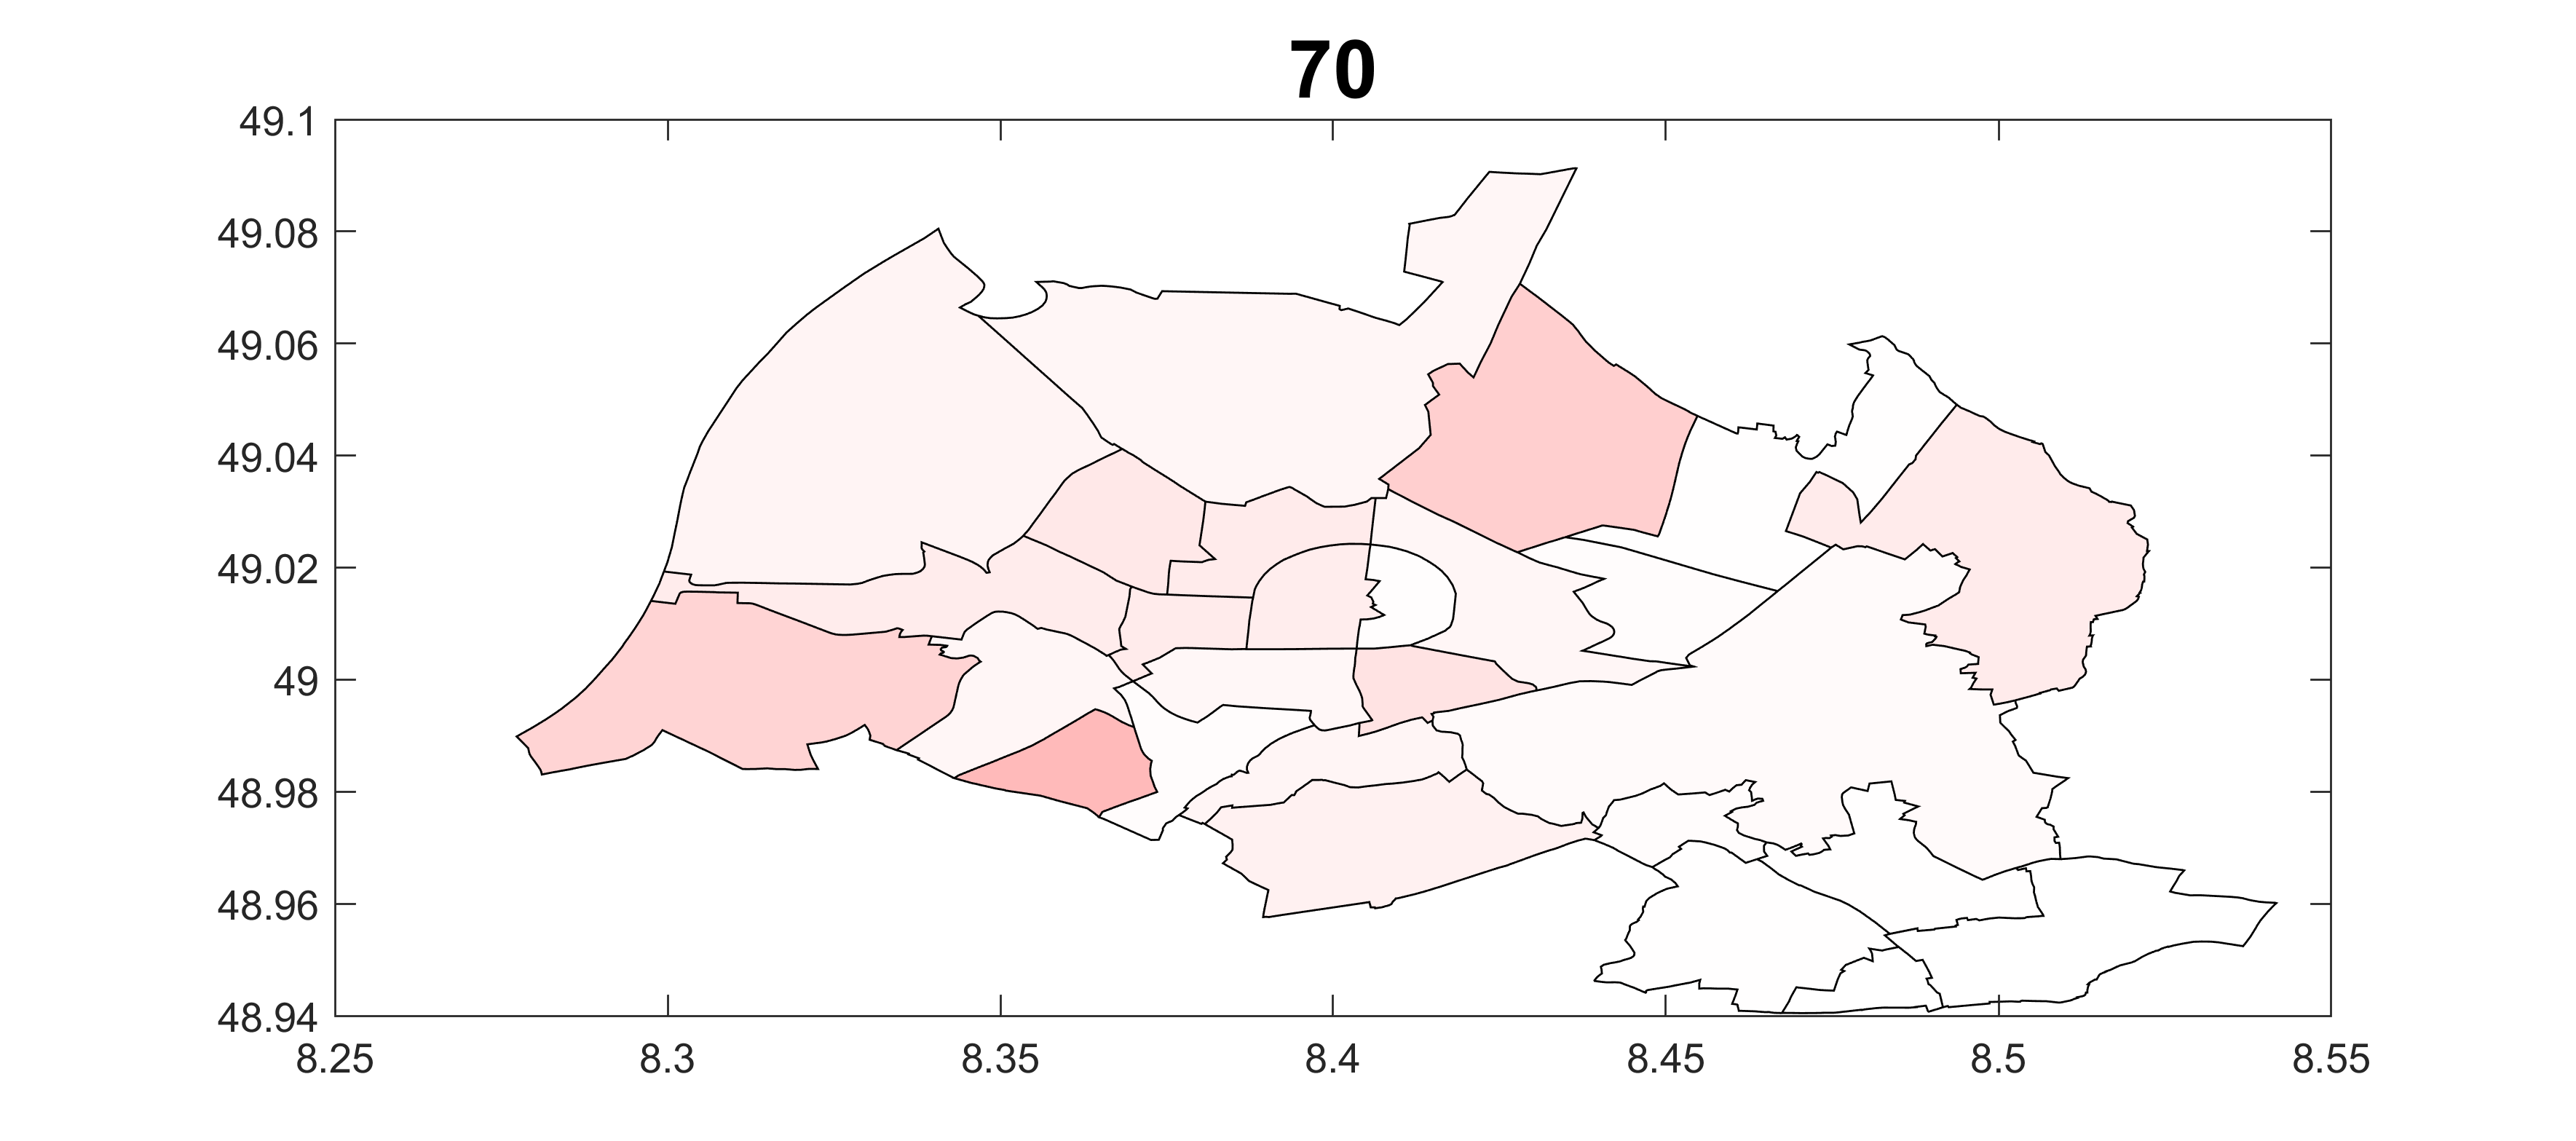
\includegraphics[width=0.3\textwidth]{bild1-70} &  
   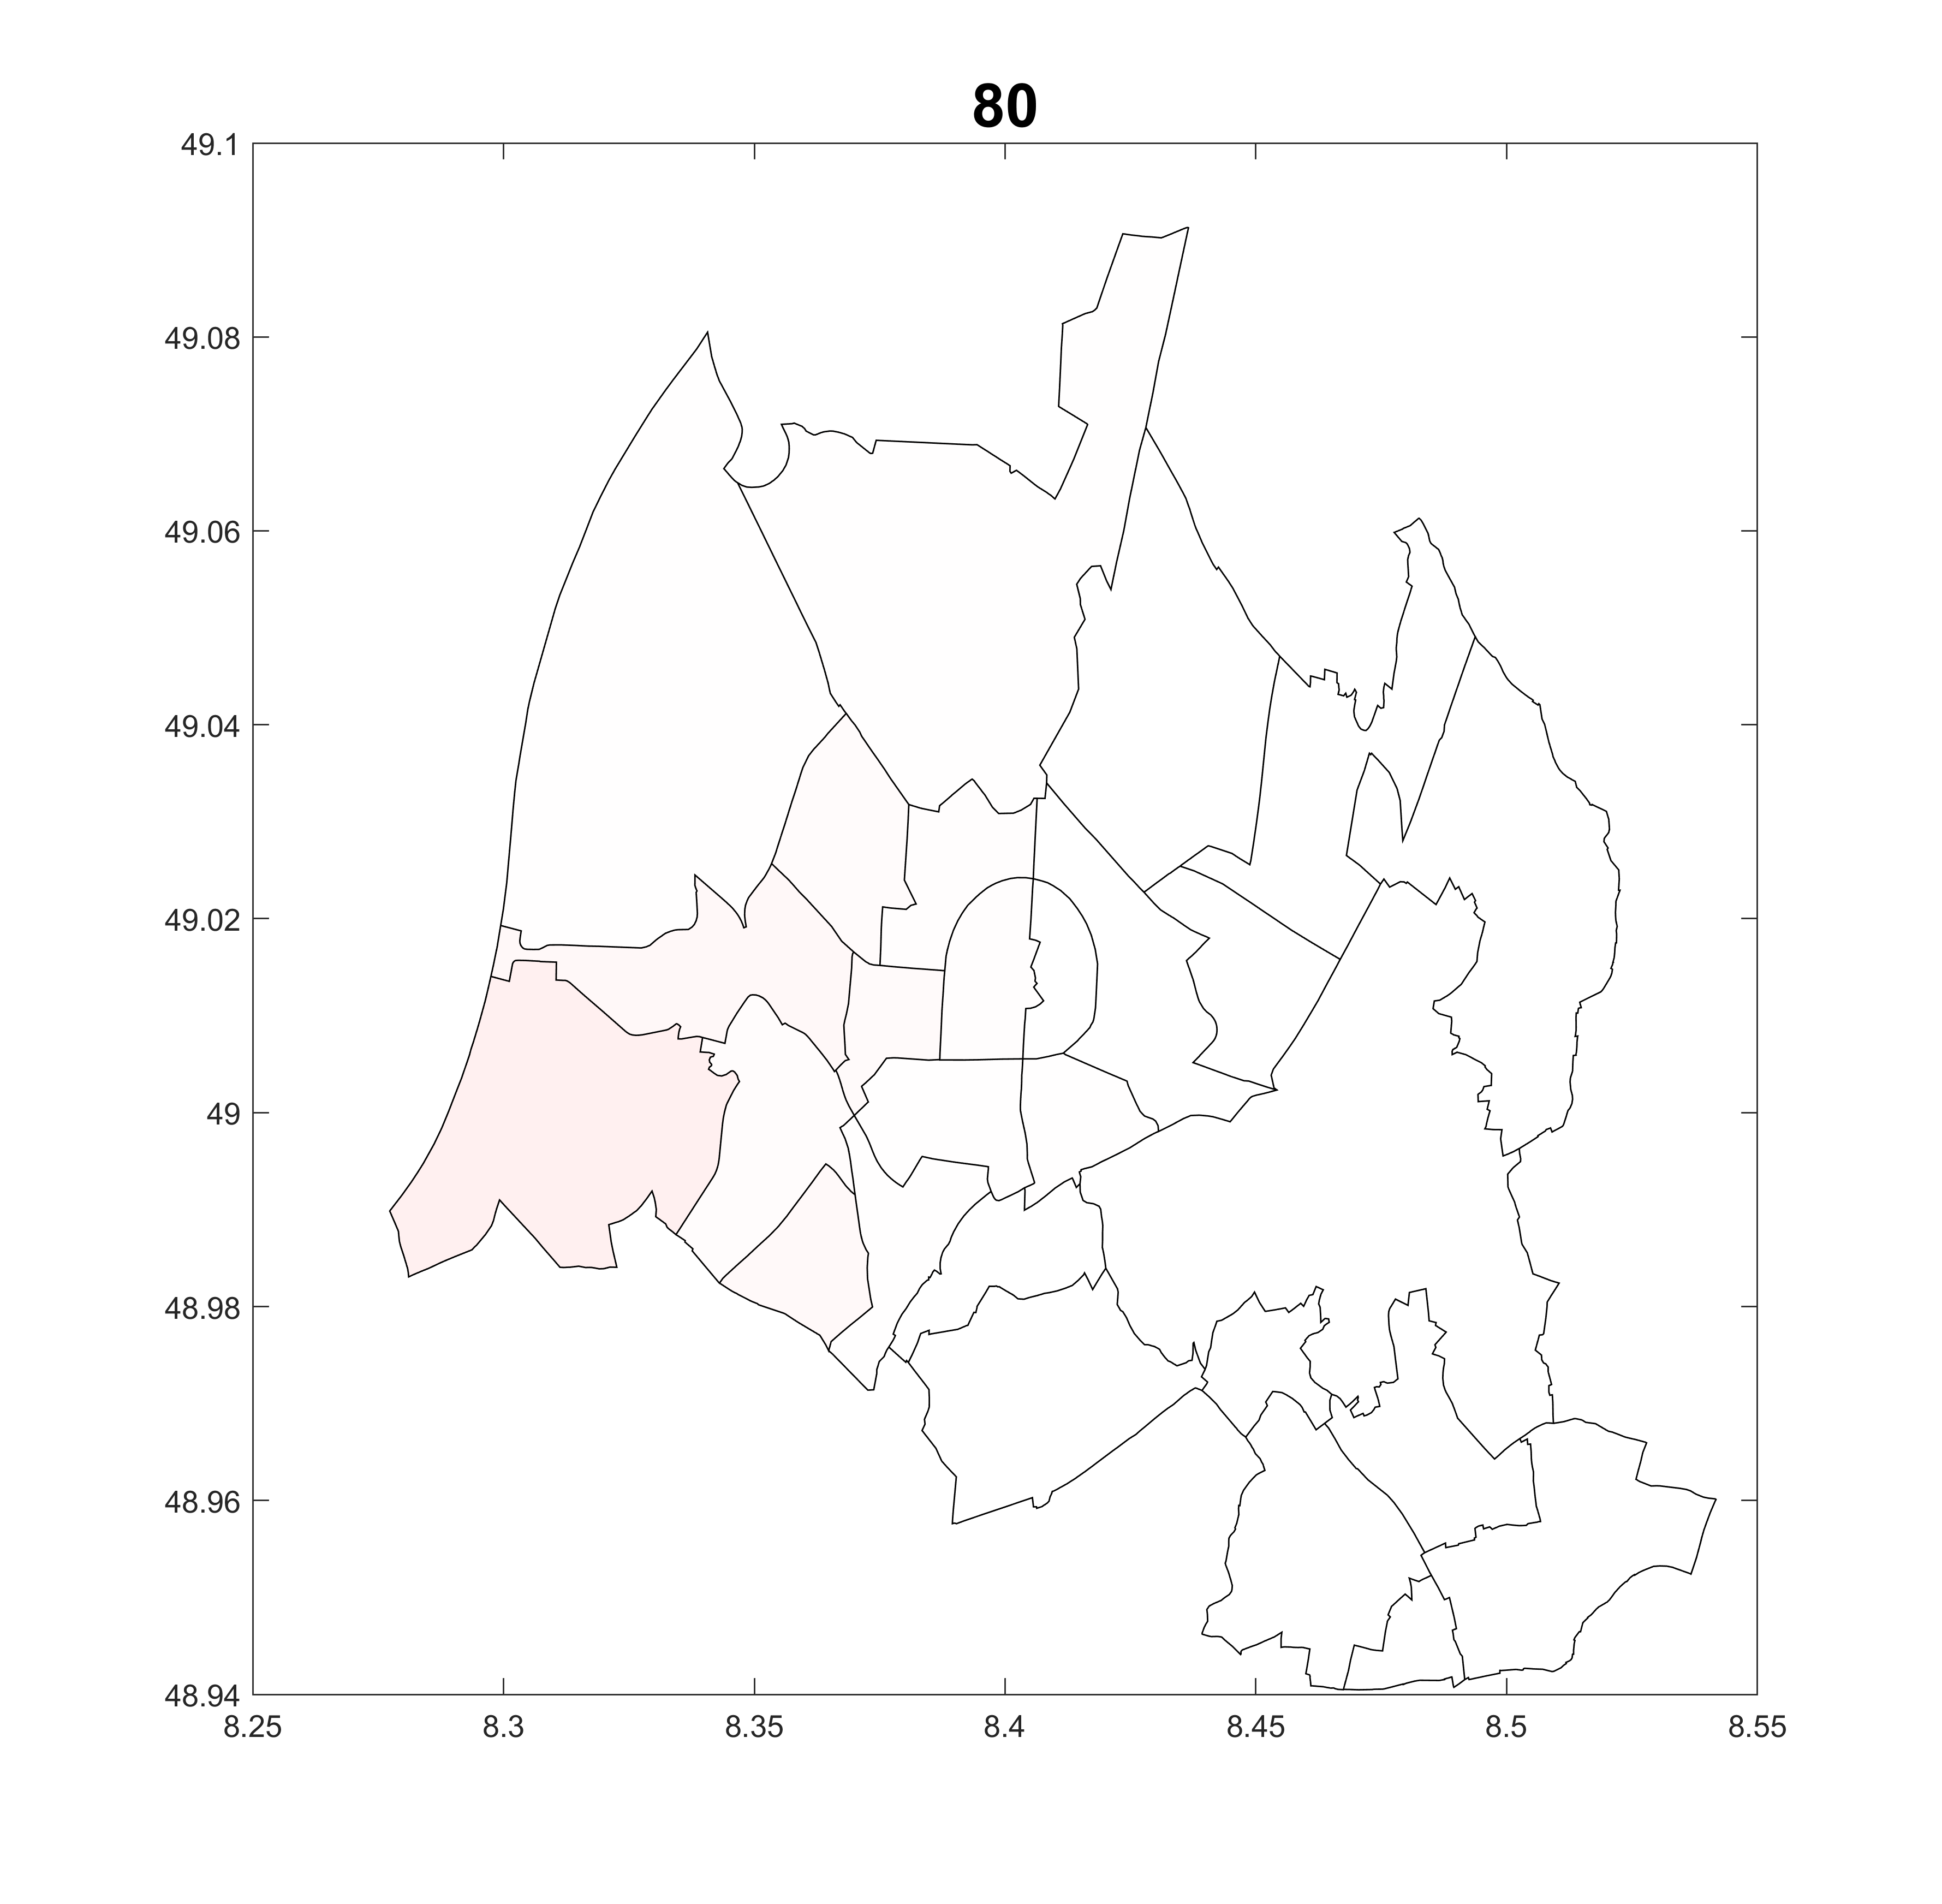
\includegraphics[width=0.3\textwidth]{bild1-80} \\
\end{tabular}
\caption{Verlauf der Krankheit zu gew\"ahlten Zeitschritten}
\end{figure}

\begin{figure}
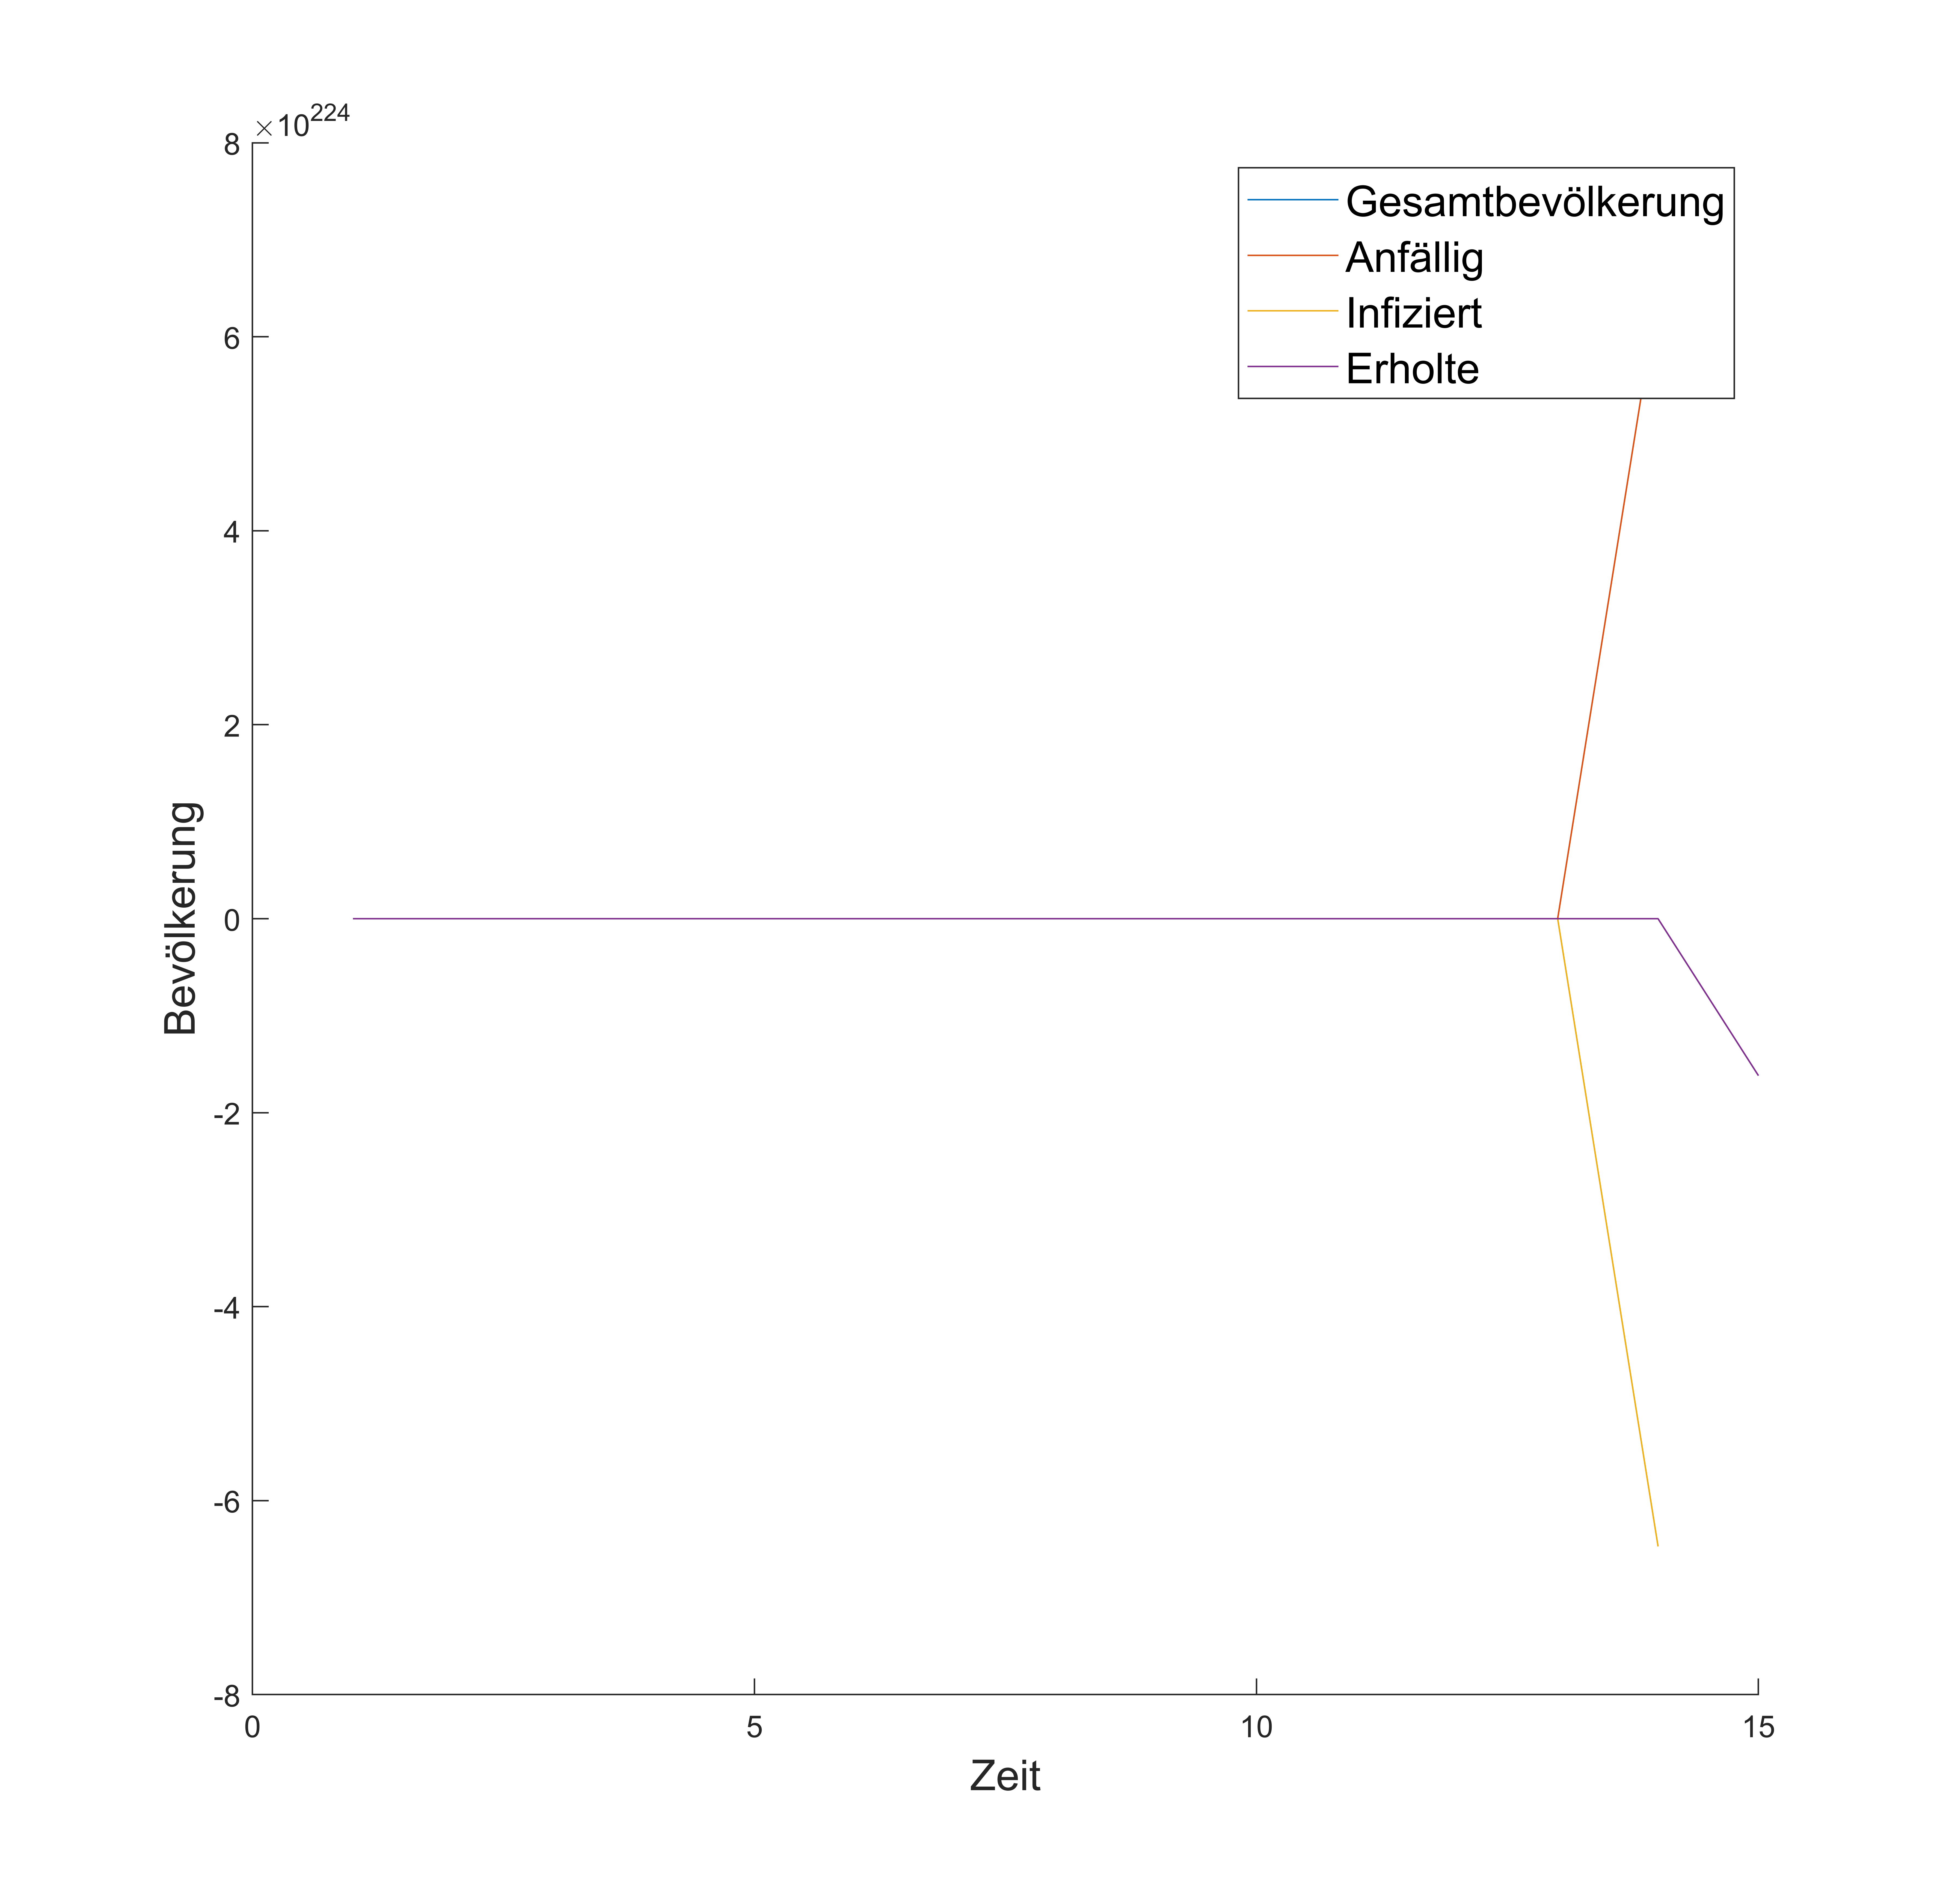
\includegraphics[width=0.5\textwidth]{bild3-1}
\caption{Krankheitsverlauf Masern}
\end{figure}

\begin{figure}
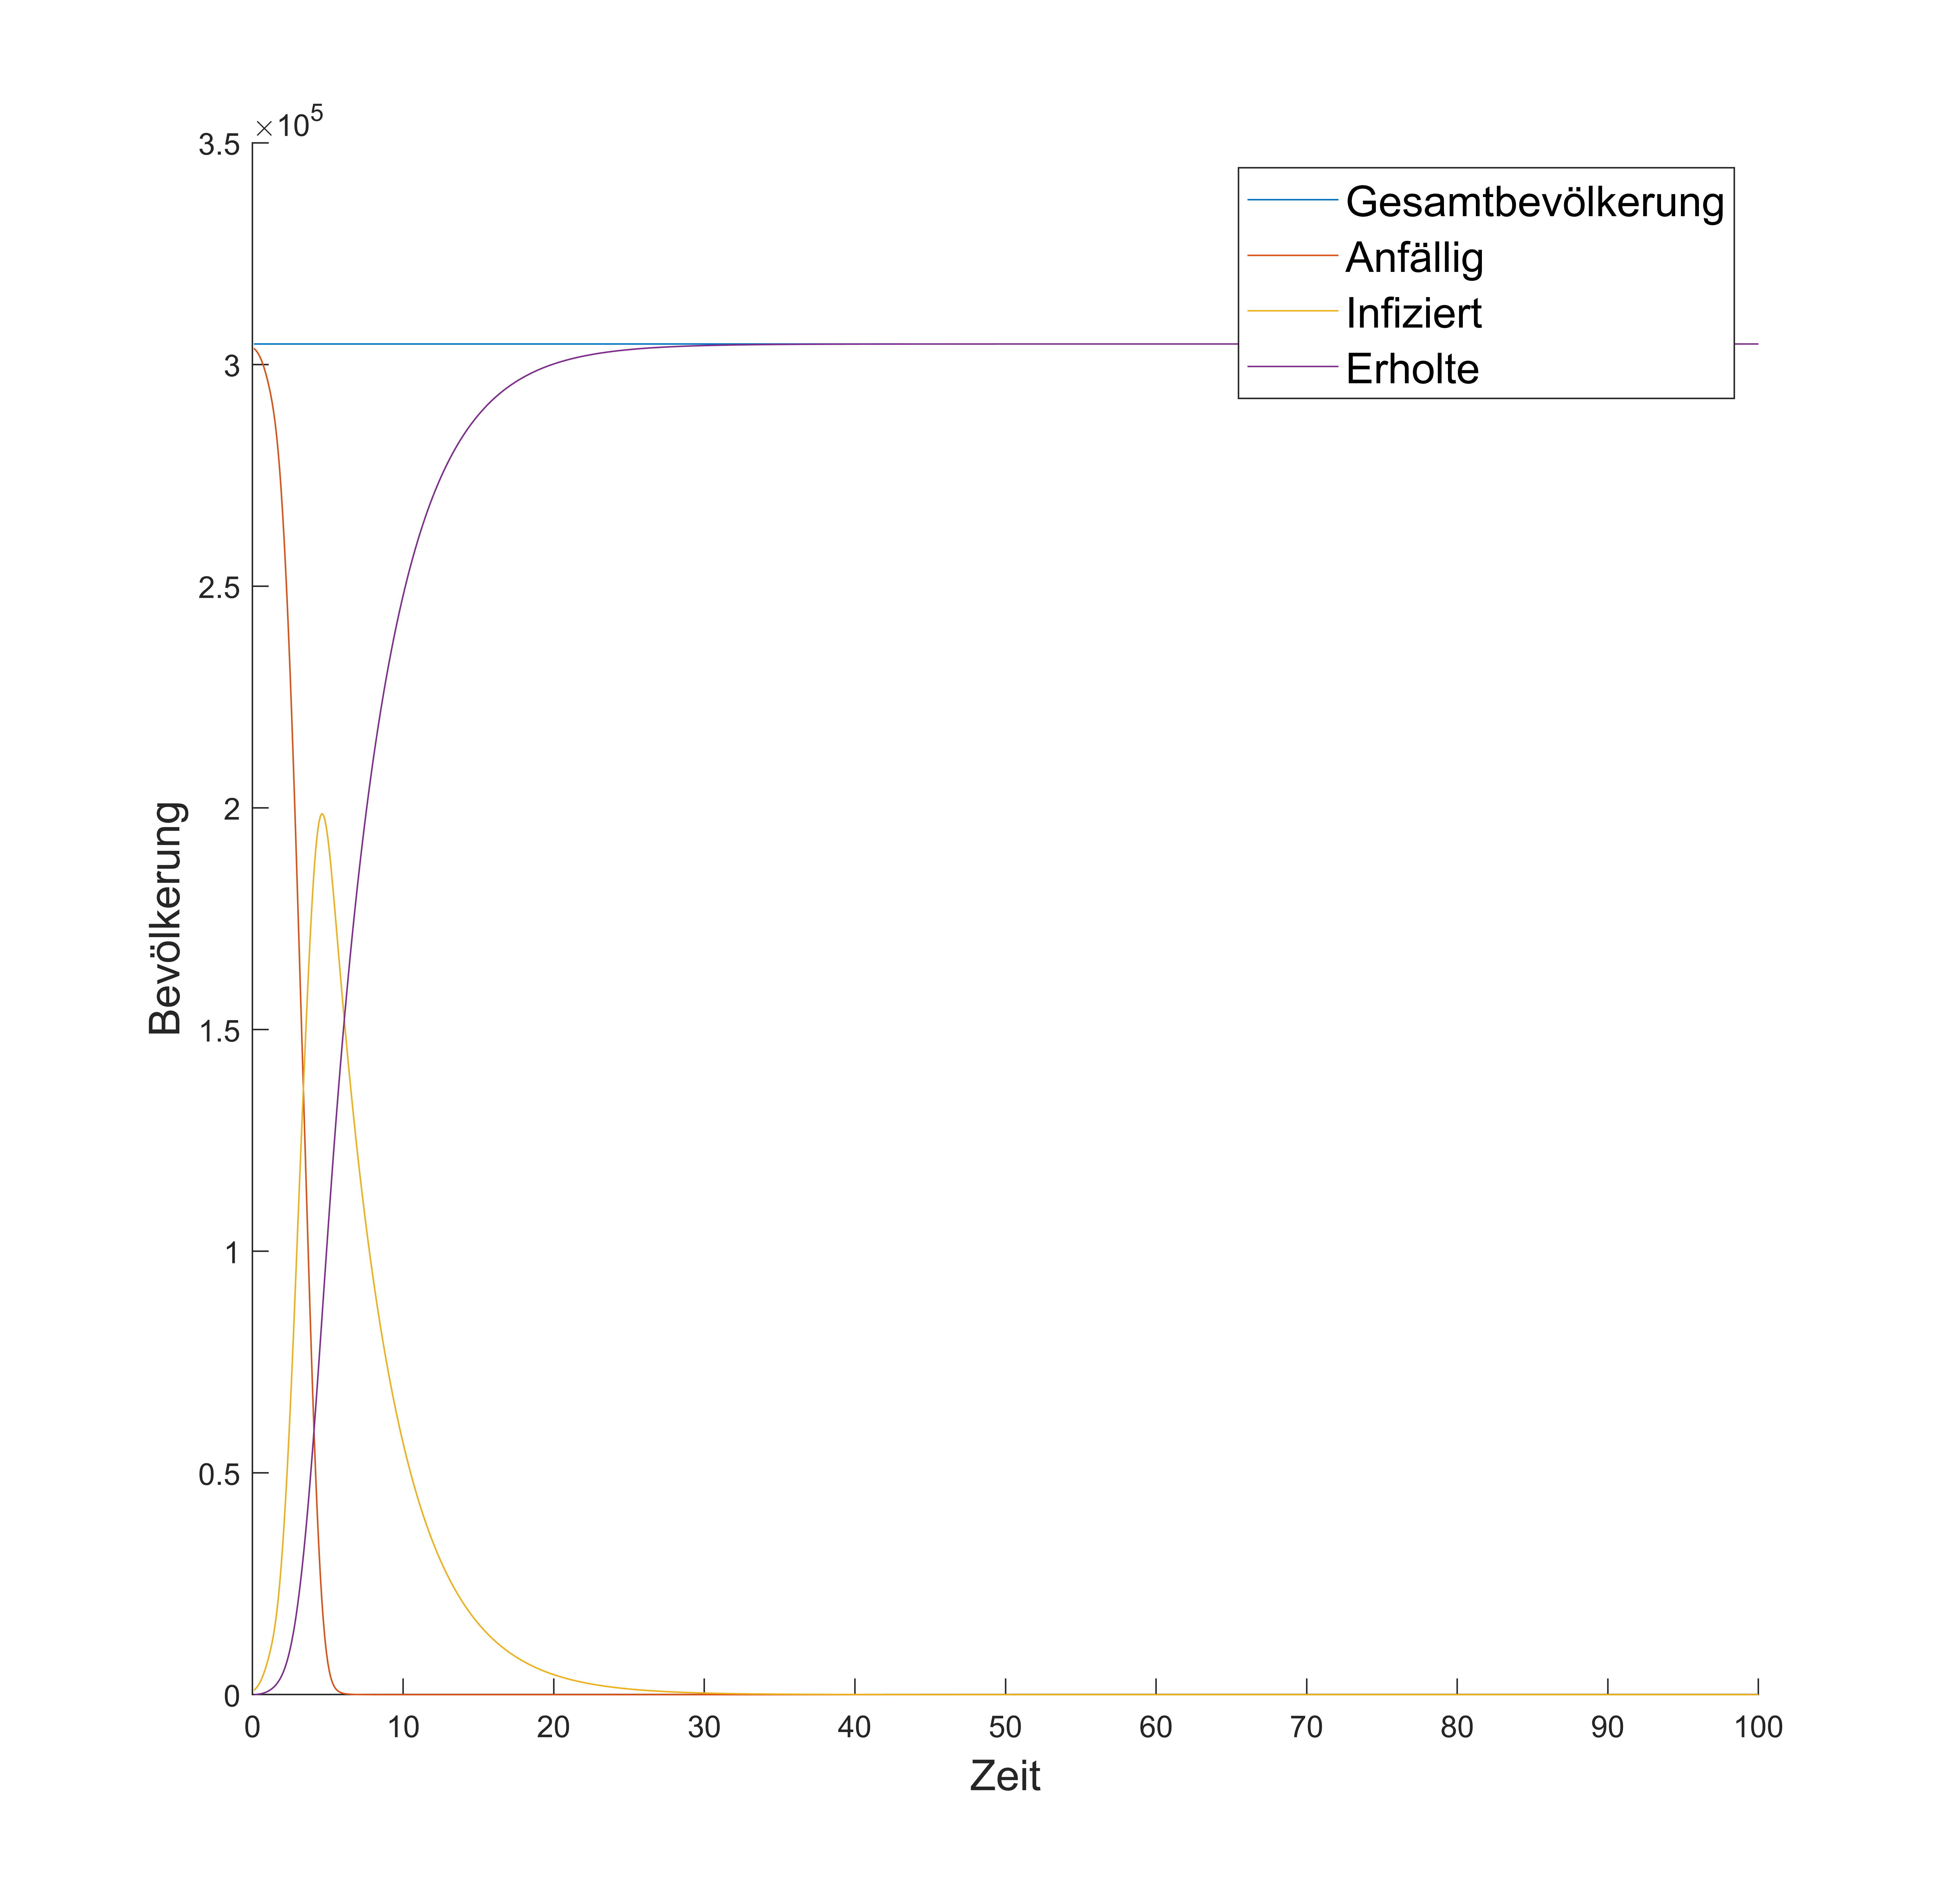
\includegraphics[width=0.5\textwidth]{bild4-1}
\caption{Krankheitsverlauf Masern mit Schrittweite 0.1}
\end{figure}
  
\end{document}
